%%
% @author : Louis Lainé 
% @contact : github.com/llaine
% 
%
% Internship report L3 MIAGE bordeaux 2013/2014. 
%
%%
\documentclass{report}

% Packages definition
%%%%%%%%%%%%%%%%%%%%%%%%%%%%%%%%%%%%%%%%%%%%%%%%%%%%%%%%%%%%%%%%%%%%%%%%%%%%%%%%%%%%%%%%%%%%%%%%%%%%%%%%%%%%%%%%%%%%%%%%%%%%%%%ù

\usepackage[utf8]{inputenc}
\usepackage[french]{babel}
\usepackage[T1]{fontenc}
\usepackage{graphics}
\usepackage{listings}
\usepackage{graphicx}
\usepackage[final]{pdfpages}
\usepackage{xcolor}
\usepackage{layout}
\usepackage[top=2cm, bottom=2cm, left=2cm, right=2cm]{geometry}
\usepackage{float}
\usepackage{titlesec, color}
\usepackage{eurosym}
\usepackage{eso-pic}
\usepackage{listings}
\usepackage{fancyhdr}
\usepackage{hyperref}

\usepackage[toc]{glossaries}



% Glossary entrys definition
%%%%%%%%%%%%%%%%%%%%%%%%%%%%%%%%%%%%%%%%%%%%%%%%%%%%%%%%%%%%%%%%%%%%%%%%%%%%%%%%%%%%%%%%%%%%%%%%%%%%%%%%%%%%%%%%%%%%%%%%%%%%%%

\newglossaryentry{seating-plan}{name={Seating-plan}, description={Plan de table. Dans le contexte du stage : plan des bureaux}}

\newglossaryentry{HR Manager}{name={HR Manager}, description={Human resource management ou directeur des ressources humaines}}

\newglossaryentry{PHP}{name={PHP}, description={Hypertext Preprocessor3, plus connu sous son sigle PHP (acronyme récursif), est un langage de programmation libre4 principalement utilisé pour produire des pages Web dynamiques via un serveur HTTP3, mais pouvant également fonctionner comme n'importe quel langage interprété de façon locale. PHP est un langage impératif orienté objet}}

\newglossaryentry{Apache}{name={Apache}, description={Le logiciel libre Apache HTTP Server (Apache) est un serveur HTTP créé et maintenu au sein de la fondation Apache. Il permet de servir des requêtes HTTP développé pour le web}}

\newglossaryentry{VM}{name={virtual Machine}, description={machine virtuelle est une illusion d'un appareil informatique créée par un logiciel d'émulation}}

\newglossaryentry{Debian}{name={Debian}, description={Distribution Linux basée sur le noyau Linux et le système GNU}}

\newglossaryentry{MySQL}{name={MySQL}, description={MySQL est un moteur de base de données relationnel écrit en PHP et open-source}}

\newglossaryentry{capacity-planning}{name={capacity-planning}, description={Gestion de la capacité. Surveillance sur le long terme de l'ensemble du parc physique afin d'éviter le dépassement d'effectif d'une manière globale sur l'agence ou d'une manière détaillé sur un floor en particulier}}

\newglossaryentry{client-serveur}{name={architecture client-serveur}, description={L'environnement client-serveur désigne un mode de communication à travers un réseau entre plusieurs programmes ou logiciels : l'un, qualifié de client, envoie des requêtes ; l'autre ou les autres, qualifiés de serveurs, attendent les requêtes des clients et y répondent. Par extension, le client désigne également l'ordinateur sur lequel est exécuté le logiciel client, et le serveur, l'ordinateur sur lequel est exécuté le logiciel serveur}}

\newglossaryentry{W3C}{name={W3C}, description={Le World Wide Web Consortium, abrégé par le sigle W3C, est un organisme de normalisation à but non lucratif, fondé en octobre 1994 chargé de promouvoir la compatibilité des technologies du World Wide Web}}

\newglossaryentry{API}{name={API}, description={En informatique, une interface de programmation (souvent désignée par le terme API pour Application Programming Interface) est un ensemble normalisé de classes, de méthodes ou de fonctions qui sert de façade par laquelle un logiciel offre des services à d'autres logiciels}}

\newglossaryentry{REST}{name={REST}, description={REST (REpresentational State Transfer) est un style d’architecture pour les systèmes hypermédia distribués, créé par Roy Fielding en 2000 dans le chapitre 5 de sa thèse de doctorat}}

\newglossaryentry{MVC}{name={MVC}, description={Le patron modèle-vue-contrôleur (en abrégé MVC, de l'anglais model-view-controller), tout comme les patrons modèle-vue-présentation ou Présentation, abstraction, contrôle, est un modèle destiné à répondre aux besoins des applications interactives en séparant les problématiques liées aux différents composants au sein de leur architecture respective}}

\newglossaryentry{MVVM}{name={MVVM}, description={Le Modèle-Vue-VueModèle (en abrégé MVVM, de l'anglais Model View ViewModel) est une architecture et une méthode de conception utilisée dans le génie logiciel. Cette méthode permet, tel le modèle MVC, de séparer la vue de la logique et de l'accès aux données en accentuant les principes de binding et d’événement}}

\newglossaryentry{framework}{name={framework}, description={En programmation informatique, un framework est un ensemble cohérent de composants logiciels structurels, qui sert à créer les fondations ainsi que les grandes lignes de tout ou d’une partie d'un logiciel (architecture)}}

\newglossaryentry{stack}{name={stack}, description={Une pile, un empilement}}

\newglossaryentry{guideline}{name={guideline}, description={Une convention, une directive, une ligne de conduite }}

\newglossaryentry{orm}{name={ORM}, description={Un mapping objet-relationnel (en anglais object-relational mapping ou ORM) est une technique de programmation informatique qui crée l'illusion d'une base de données orientée objet à partir d'une base de données relationnelle en définissant des correspondances entre cette base de données et les objets du langage utilisé. On pourrait le désigner par « correspondance entre monde objet et monde relationnel »}}

\newglossaryentry{versionning}{name={versionning}, description={Un logiciel de gestion de versions (ou VCS en anglais, pour Version Control System) est un logiciel qui permet de stocker un ensemble de fichiers en conservant la chronologie de toutes les modifications qui ont été effectuées dessus. Il permet notamment de retrouver les différentes versions d'un lot de fichiers connexes}}

\newglossaryentry{jQuery UI}{name={jQuery UI}, description={Bibliothèque de widgets graphiques, d'animations visuelles Javascript }}

\newglossaryentry{MongoDB}{name={MongoDB}, description={MongoDB (de l'anglais humongous qui peut être traduit par « énorme ») est un système de gestion de base de données orientée documents, répartissable sur un nombre quelconque d'ordinateurs et ne nécessitant pas de schéma prédéfini des données}}

\newglossaryentry{big data}{name={big data}, description={Les big data, littéralement les « grosses données », parfois appelées données massives, est une expression anglophone utilisée pour désigner des ensembles de données qui deviennent tellement volumineux qu'ils en deviennent difficiles à travailler avec des outils classiques de gestion de base de données ou de gestion de l'information}}

\newglossaryentry{cluster}{name={cluster}, description={Un cluster est une grappe de serveurs (ou « ferme de calcul ») constituée de deux serveurs au minimum (appelés aussi nœuds) et partageant une baie de disques commune}}

\newglossaryentry{scalabilité}{name={scalabilité}, description={En informatique matérielle et logicielle et en télécommunications, la scalability ou scalabilité (calque de traduction) désigne la capacité d'un produit à s'adapter à un changement d'ordre de grandeur de la demande (montée en charge), en particulier sa capacité à maintenir ses fonctionnalités et ses performances en cas de forte demande}}

\newglossaryentry{SGBDR}{name={SGBDR}, description={Un système de gestion de base de données (abr. SGBD) est un logiciel système destiné à stocker et à partager des informations dans une base de données, en garantissant la qualité, la pérennité et la confidentialité des informations, tout en cachant la complexité des opérations}}

\newglossaryentry{NoSQL}{name={NoSQL}, description={NoSQL (Not only SQL en anglais) désigne une catégorie de systèmes de gestion de base de données (SGBD) qui n'est plus fondée sur l'architecture classique des bases relationnelles. L'unité logique n'y est plus la table, et les données ne sont en général pas manipulées avec SQL}}

\newglossaryentry{asynchrone}{name={asynchrone}, description={L’asynchronisme désigne le caractère de ce qui ne se passe pas à la même vitesse, que ce soit dans le temps ou dans la vitesse proprement dite, par opposition à un phénomène synchrone}}

\newglossaryentry{KPI}{name={KPI}, description={Les indicateurs clefs de performance (ICP), ou en anglais Key Performance Indicators (KPI) , sont des indicateurs mesurables d'aide décisionnelle}}

\newglossaryentry{SonarQube}{name={SonarQube}, description={SonarQube (précédemment Sonar) est un logiciel libre permettant de mesurer la qualité du code source en continu}}

\newglossaryentry{NGiNX}{name={NGiNX}, description={Nginx [engine x] est un logiciel libre de serveur Web (ou HTTP) ainsi qu'un proxy inverse écrit par Igor Sysoev, dont le développement a débuté en 2002 pour les besoins d'un site russe à très fort trafic}}

\newglossaryentry{HTTP}{name={HTTP}, description={L'HyperText Transfer Protocol, plus connu sous l'abréviation HTTP — littéralement « protocole de transfert hypertexte » — est un protocole de communication client-serveur développé pour le World Wide Web}}

\newglossaryentry{full stack}{name={full stack}, description={Full Stack désigne le fait d'utiliser l'ensemble des couches d'un applicatif métier utilisant la même logique. Ici on parle de Full Stack dans le sens ou toutes les couches de l'application utilise le langage JavaScript}}

\newglossaryentry{drag'n'drop}{name={drag'n'drop}, description={Drapg'n'drop ou glisser-déposer est dans une interface graphique une méthode consistant à utiliser une souris, pavé ou écran, pour déplacer d'un endroit à un autre un élément graphique présent sur l'écran d'un smartphone, tablette ou ordinateur}}

\newglossaryentry{intégration continue}{name={intégration continue}, description={L'intégration continue est un ensemble de pratiques utilisées en génie logiciel consistant à vérifier à chaque modification de code source que le résultat des modifications ne produit pas de régression dans l'application développée}}

\newglossaryentry{SSH}{name={SSH}, description={Secure Shell (SSH) est à la fois un programme informatique et un protocole de communication sécurisé. Le protocole de connexion impose un échange de clés de chiffrement en début de connexion}}

\newglossaryentry{extremme programming}{name={extremme programming}, description={En informatique et plus particulièrement en génie logiciel, Extreme Programming (XP) est une méthode agile plus particulièrement orientée sur l'aspect réalisation d'une application, sans pour autant négliger l'aspect gestion de projet. XP est adapté aux équipes réduites avec des besoins changeants. XP pousse à l'extrême des principes simples}}

\newglossaryentry{Jenkins}{name={Jenkins}, description={Jenkins est un outil open source d'intégration continue, fork de l'outil Hudson après les différends entre son auteur, Kohsuke Kawaguchi, et Oracle. Écrit en Java, Jenkins fonctionne dans un conteneur de servlets tel qu’Apache Tomcat, ou en mode autonome avec son propre serveur Web embarqué}}

\newglossaryentry{patch}{name={patch}, description={Un patch ou correctif est une section de code que l'on ajoute à un logiciel, pour y apporter des modifications : correction d'un bug, traduction, crack}}

\newglossaryentry{CTO}{name={CTO}, description={Le directeur de la technologie (CTO, pour Chief Technology Officer en anglais) est un employé chargé de s'occuper de la direction des questions scientifiques et techniques au sein d'une organisation}}

\newglossaryentry{moteur V8}{name={moteur v8 javascript}, description={V8 JavaScript engine est un moteur JavaScript open source développé par Google au Danemark. Il est notamment utilisé dans les navigateurs Internet Google Chrome et Chromium}}



% Packages modification, command definition
%%%%%%%%%%%%%%%%%%%%%%%%%%%%%%%%%%%%%%%%%%%%%%%%%%%%%%%%%%%%%%%%%%%%%%%%%%%%%%%%%%%%%%%%%%%%%%%%%%%%%%%%%%%%%%%%%%%%%%%%%%%%%%%ù

\makeglossaries


\pdfminorversion=5 
\pdfcompresslevel=9
\pdfobjcompresslevel=10

\newcommand{\jumpOne}{\\[1\baselineskip]}
\newcommand{\jumpTwo}{\\[2\baselineskip]}

\pagestyle{fancy}

% Modification des styles de chapitres
\definecolor{gray75}{gray}{0.75}
\newcommand{\hsp}{\hspace{12pt}}
\titleformat{\chapter}[hang]{\Huge\bfseries}{\thechapter\hsp\textcolor{gray75}{|}\hsp}{0pt}{\Huge}

\definecolor{RedOrange}{rgb}{255, 99, 71}
\definecolor{Red}{rgb}{192,192,192}
\definecolor{DarkSkyBlue}{HTML}{204A87}


\hypersetup{
     colorlinks  = true,
     citecolor   = DarkSkyBlue,
     linkcolor   = DarkSkyBlue,
     urlcolor 	 = DarkSkyBlue
}

% Redefinition des section/sub
\titleformat*{\section}{\Large\bfseries\sffamily\color{gray}}
\titleformat*{\subsection}{\large\bfseries\sffamily\color{gray}}
\titleformat*{\subsubsection}{\itshape\large\sffamily\color{gray}}


\newcommand{\HRule}{\rule{\linewidth}{0.5mm}}

% BACKGROUND PICTURES 
\newcommand{\backgroundMain}{
	\put(0,0){
		\parbox[b][\paperheight]
		{\paperwidth}{%
			\vfill
			\centering
			
\includegraphics[
			width=\paperwidth,
			height=\paperheight,
			]{assets/accueil.png}%
			\vfill
		}
	}
}


% Definition du header && footer 
\renewcommand{\headrulewidth}{1.5pt}
\fancyhead[C]{}
\fancyhead[L]{\usefont{OT1}{phv}{m}{n} Année 2013/2014}
\fancyhead[R]{\usefont{OT1}{phv}{m}{n} Louis Lainé}

\renewcommand{\footrulewidth}{1pt}
\fancyfoot[C]{\textbf{\thepage}} 
\fancyfoot[L]{
\includegraphics[keepaspectratio=true,width=3cm]{assets/logo_bdx.jpg}}
\fancyfoot[R]{
\includegraphics[keepaspectratio=true,width=1.5cm]{assets/logo.png}}

\definecolor{mygreen}{rgb}{0,0.6,0}
\definecolor{mygray}{rgb}{0.5,0.5,0.5}
\definecolor{mymauve}{rgb}{0.58,0,0.82}

\definecolor{lightgray}{rgb}{.9,.9,.9}
\definecolor{darkgray}{rgb}{.4,.4,.4}
\definecolor{purple}{rgb}{0.65, 0.12, 0.82}


\lstset{
	basicstyle=\small\sffamily,
	numbers=left,
	numberstyle=\tiny,
	frame=tb,
	columns=fullflexible,
	showstringspaces=false,
	commentstyle=\color{mygreen},
	keywordstyle=\color{blue},
	stringstyle=\color{mymauve}
}

 % JavaScript definition on lstlisting
\lstdefinelanguage{JavaScript}{
  keywords={typeof, new, true, false, catch, function, return, null, catch, switch, var, if, in, while, do, else, case, break},
  keywordstyle=\color{blue}\bfseries,
  ndkeywords={class, export, boolean, throw, implements, import, this},
  ndkeywordstyle=\color{darkgray}\bfseries,
  identifierstyle=\color{black},
  sensitive=false,
  comment=[l]{//},
  morecomment=[s]{/*}{*/},
  commentstyle=\color{purple}\ttfamily,
  stringstyle=\color{red}\ttfamily,
  morestring=[b]',
  morestring=[b]"
}

% UTF8 remplacement for lstlisting
\lstset{inputencoding=utf8,extendedchars=true,literate={á}{{\'a}}1 {ã}{{\~a}}1 {é}{{\'e}}1,numbers=left, showstringspaces=false ,stepnumber=2,firstnumber=1} 


% Title page
%%%%%%%%%%%%%%%%%%%%%%%%%%%%%%%%%%%%%%%%%%%%%%%%%%%%%%%%%%%%%%%%%%%%%%%%%%%%%%%%%%%%%%%%%%%%%%%%%%%%%%%%%%%%%%%%%%%%%%%%%%%%%%%ù

\begin{document}

% Page de garde
\begin{titlepage}

\AddToShipoutPicture*{\backgroundMain}

\begin{center}

\noindent

\begin{minipage}{.5\textwidth}
	\begin{flushleft}
		
\includegraphics[width=0.5\textwidth]{assets/logo.png}~\\[1cm]
		\usefont{OT1}{phv}{m}{n}
		\begin{description}
			\item Arnaud Roudsovsky
			\item Christophe Frezier
		\end{description}
		
	\end{flushleft}
\end{minipage}% 
\begin{minipage}{.5\textwidth}
	\begin{flushright}
		
\includegraphics[width=0.6\textwidth]{assets/miage_bordeaux.jpg}~\\[1cm]
		\usefont{OT1}{phv}{m}{n}
		Jean Luc Le Gual
	\end{flushright}
\end{minipage}

\\[15\baselineskip] 

\begin{flushleft}
	\usefont{OT1}{phv}{m}{n}
	\Large {\color{red}Analyste développeur au sein de la cellule d'expertise technique}
\end{flushleft}
	\par
		\hrule height 2pt
	\par
\begin{flushright}
	\usefont{OT1}{phv}{m}{n}
		\Large Lainé Louis
	\par
\end{flushright}
\vspace*{\fill}

% Bottom of the page
\usefont{OT1}{phv}{m}{n}
{\large Université de Bordeaux. }

\end{center}

\end{titlepage}

% Main document 
%%%%%%%%%%%%%%%%%%%%%%%%%%%%%%%%%%%%%%%%%%%%%%%%%%%%%%%%%%%%%%%%%%%%%%%%%%%%%%%%%%%%%%%%%%%%%%%%%%%%%%%%%%%%%%%%%%%%%%%%%%%%%%%ù
\setlength{\parindent}{0cm}
\usefont{OT1}{phv}{m}{n} % Choix de la police pour l'ensemble du txt

% PAGE DE REMERCIEMENTS
\chapter{Remerciements}
En premier lieu, je souhaite adresser mes plus sincères remerciements à l'ensemble de l'équipe SQLI Bordeaux. 
\jumpOne
J'ai particulièrement apprécié le professionnalisme et la bonne humeur de chacun, qualités qui ont fait de ce stage une réussite tant sur le plan humain que professionnel. 
\jumpOne
Je tiens à remercier chaleureusement, \textbf{Béatrice Fichera} et \textbf{Emmanuel Uria} qui m'ont accordés leur confiance et permis d'intégrer l'agence de Bordeaux pour ce stage.
\jumpOne
Je souhaite également remercier \textbf{Arnaud Roudsovsky}, mon maitre de stage, ainsi que toute l'équipe d'experts techniques avec laquelle j'ai été amené à travailler.
\jumpOne
Merci à \textbf{Miguel Diez Garcia}, \textbf{Frédéric Gracia}, \textbf{Romain Ballan}, \textbf{Christian Alonzo Chavez Ley}, \textbf{Rodolphe Baron} pour leurs conseils. 
\jumpOne
Un merci en particulier à \textbf{Christophe Frezier} qui m'a guidé, aidé et conseillé tout particulierement durant ce stage. 
\jumpOne
Un merci à Mr \textbf{Jean-Luc Le Gual} pour sont suivi pendant le stage et ses conseils ainsi que l'équipe pédagogique de la MIAGE Bordeaux, qui m'a permis par le biais de ce stage, d'enrichir mon experience profesionnelle.   





\newpage






% PAGE DE SOMMAIRE
\tableofcontents{}

\newpage
% RESUME EN ANGLAIS
\chapter{Summary}

To validate my bachelor degree in computing science i had to make an intership for 3 month which a decided to perform in a IT service company named SQLI located near Bordeaux at Pessac.

The main goal of the internship is to enforce all the courses seen during the year like project management or application developpement. 

During 3 month i worked in the technical expertise center under the direction of the CTO Mr Roudsovsky Arnaud. 

He give me those internship topics.
\begin{itemize}
	\item Analysis and developpement of a management tool in order to manage the agency seating-plan. 
	\item Analysis and developpement of an application in order to aggregate project key's perfomance indicator in an decision support application. 
\end{itemize}

Those topic, were perfectly in harmony with my professionnal project which is working with a very heavy technical aspect. 
\jumpOne
Now i'm going to introduce the followings parts.
\begin{itemize}
	\item Firstly i'm going to introduce the firm.
	\item Secondly i'm going to explain how i led my first internship topic
	\item Thridly i'm going to describe how i led the second internship topic 
	\item And finally i'm going to present the teachings learned.   
\end{itemize} 






\newpage






% INTRODUCTION
\chapter{Introduction}

\section{Le groupe SQLI}

\subsection{Présentation et histoire}
Le groupe SQLI a une expertise reconnue dans la conception et la mise en œuvre de systèmes
d’informations reposant sur les nouvelles technologies. Il accompagne ses clients quotidiennement à
divers niveaux : du conseil en amont du projet au transfert de compétences en aval, en passant par la
réalisation, l’intégration et la maintenance des applications.
\jumpOne
SQLI est également la première SSII européenne à avoir mis en pratique le modèle CMMI
(Capability Maturity Model Integration) et la première à avoir été certifiée CMMI niveau 3. Ce
modèle permet au groupe de garantir à ses clients un certain niveau de qualité dans ses projets.
Cette double orientation d'innovation et de qualité a permis à SQLI de devenir un leader européen dans le
domaine des services utilisant Internet et les nouvelles technologies informatiques.
\jumpOne
La société créee en 1990 et le schéma ci dessous rappelle les principales étapes de l'évolution de l'entreprise lui ayant permis d'aboutir au stade actuel de développement. 
\begin{figure}[h!]
	\centering
	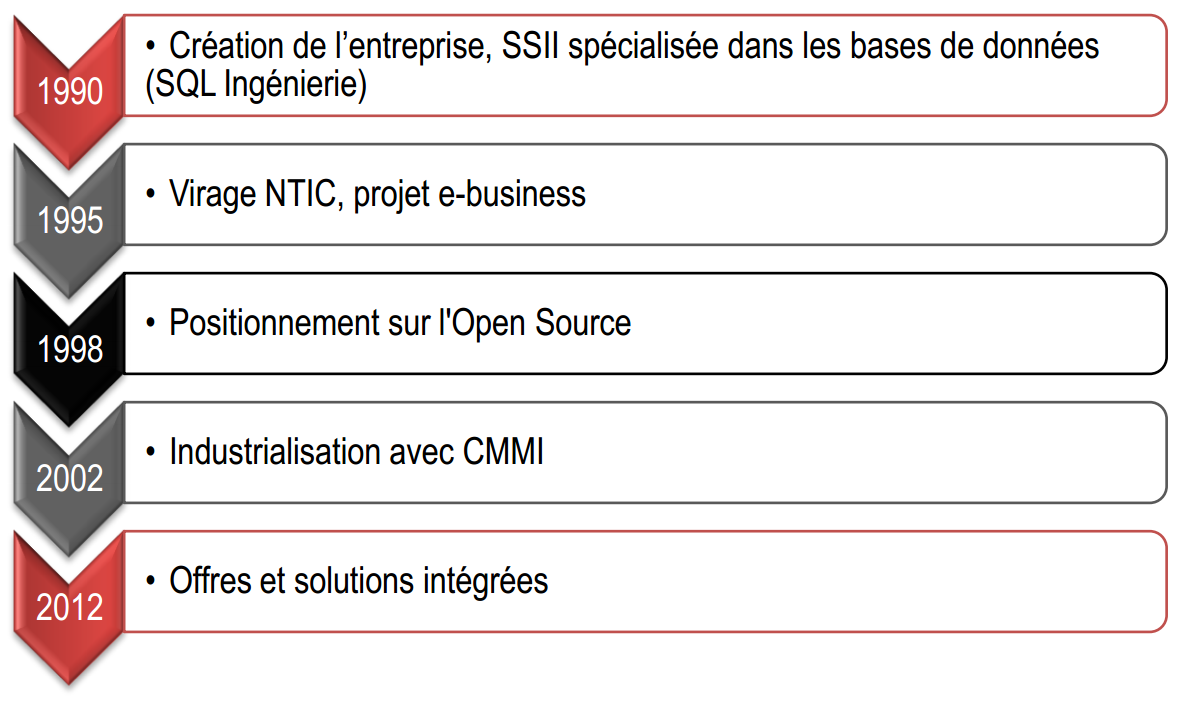
\includegraphics[width=0.7\textwidth]{assets/timeline.png}
	\caption{Historique de la société}
\end{figure}

\subsection{Un groupe européen}

Le groupe SQLI emploie aujourd’hui plus de 1800 collaborateurs dans 17 sites répartis en France, en
Suisse, dans les pays du Benelux et au Maroc.
Fondée il y a onze ans, l’agence SQLI de Bordeaux a connu une forte croissance ces dernières
années pour compter aujourd’hui environ 150 collaborateurs. L’agence de Bordeaux est donc de
taille respectable, et comporte tous les pôles du groupe que sont l’intégration, le consulting, l’agence web et la cellule d'expertise technique au sein duquel j’ai effectué mon stage.
\jumpTwo

\subsection{Les valeurs et le positionnement de l'entreprise}
Pour se démarquer de la concurrence, SQLI se développe autours de 4 axes majeurs. 
\jumpOne

\begin{figure}[h!]
	\centering
	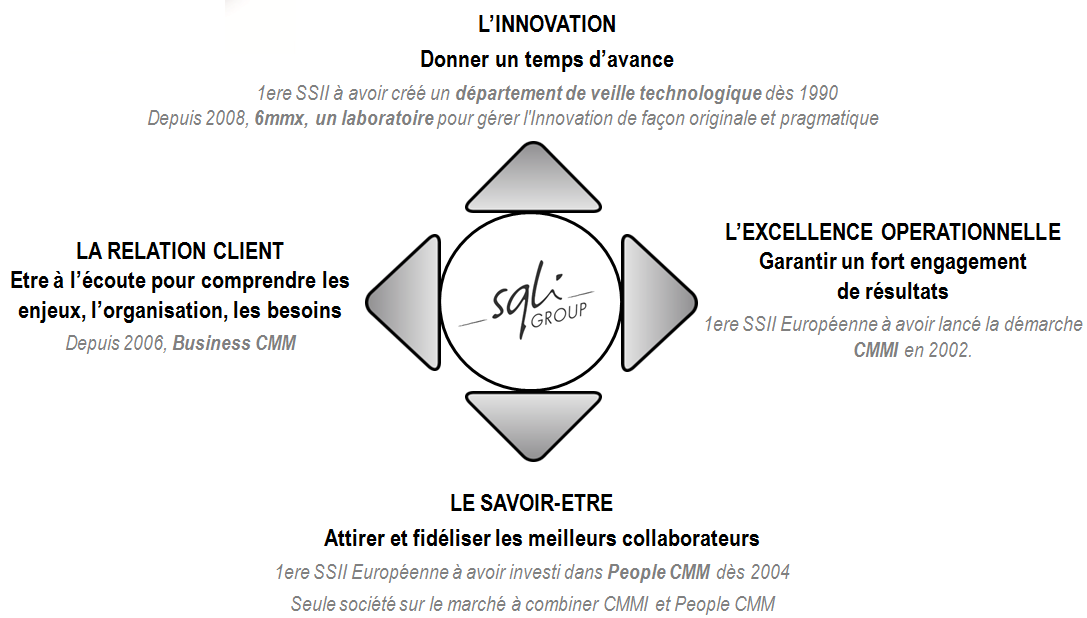
\includegraphics[width=0.7\textwidth]{assets/valeurs.png}
	\caption{Les valeurs de la société}
\end{figure}


Une des ambitions du groupe est de renforcer ses compétences par des acquisitions ou en nouant des partenariats industriels et commerciaux afin de développer des solutions métiers e-business innovantes dans des secteurs très porteurs. \\ 
Ainsi parmi les entreprises ayant rejoint récemment le groupe SQLI :

\begin{description}
	\item[INLOG]{Secteur de la santé} 
	\item[IconeWeb]{Secteur de l'immobilier} 
	\item[Clear Value]{Spécialiste français de SAP} 
\end{description}





\newpage





\subsection{Les métiers}
SQLI souhaite pouvoir être un interlocuteur pertinent quelque soit les besoins du client, c’est pourquoi elle regroupe de nombreuses activitées.

\begin{figure}[h!]
	\centering
	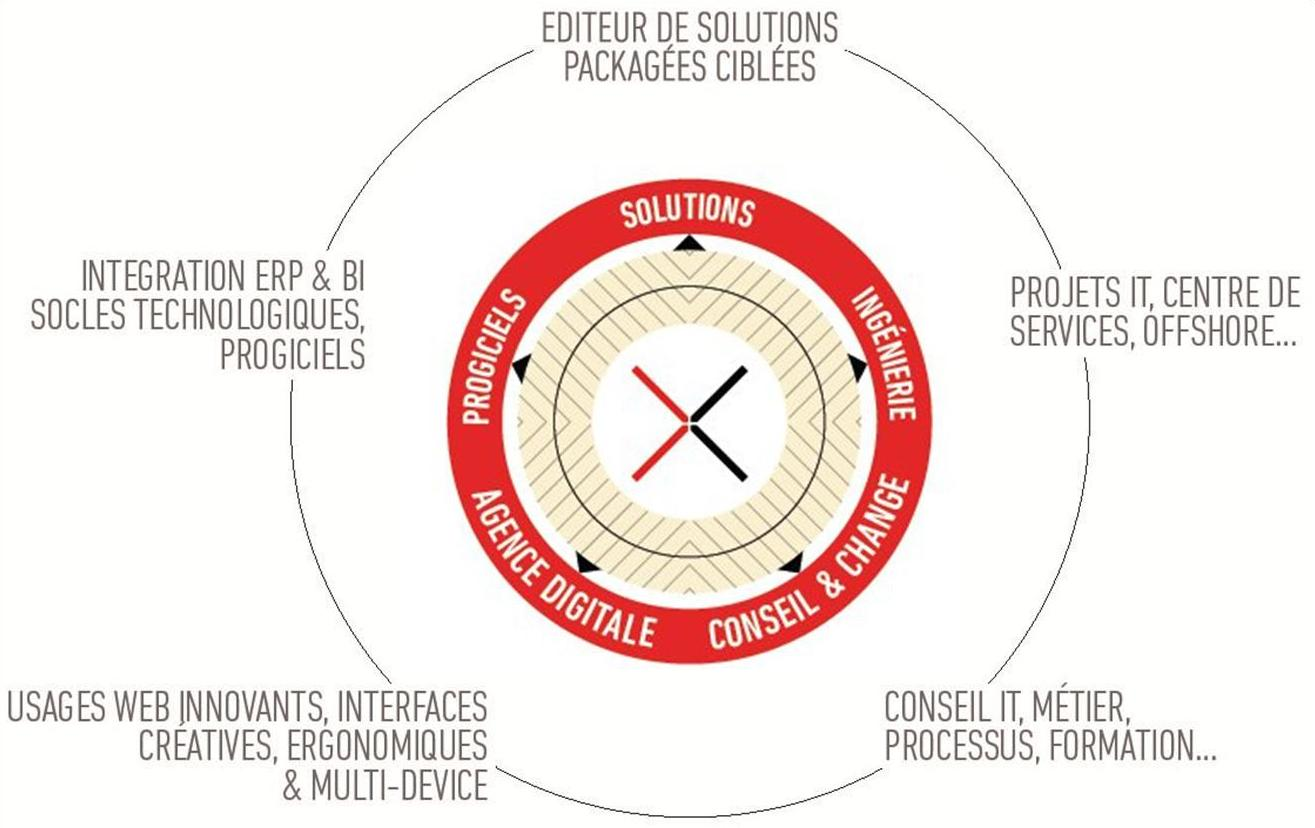
\includegraphics[width=0.7\textwidth]{assets/metiers.jpg}
	\caption{Les métiers de SQLI}
\end{figure}

\subsubsection{Le pôle solutions}
Le groupe vend ses propres applications de logistique, finance, management de projet, dont la suite
SteeringProject, orientée gestion de projet et maintenance applicative.

\subsubsection{Le pôle ingénierie}
Le groupe affiche une expertise reconnue dans le développement d’applications reposant sur les
nouvelles technologies (J2EE 3 , PHP, .Net, Oracle, SQL Server, et autres). Ceci permet à ses ingénieurs
d'améliorer leurs expertises dans ces domaines en mettant en œuvre essentiellement des projets web.

\subsubsection{Le pôle conseil et change}
Le conseil en système d’information permet d’offrir des services d'aide pour la mise en place de
systèmes d’informations. Ces conseils peuvent porter autant sur le plan décisionnel ou technologique
que sur le plan fonctionnel. Ce pôle apporte au client une aide opérationnel qui vise à définir des
solutions personnalisées en intégrant les différentes contraintes du système d’information. Il va aussi
donner des préconisations et des aides quant au choix technique pour la mise en place de nouvelles
solutions.

\subsubsection{Le pôle agence digitale}
SQLI Agency est spécialisé dans le design d'apllication web. Elle propose à ses clients des réponses à forte valeur ajoutée : conseil en performance ergonomique, connaissance utilisateur, ainsi que des prestations de création, de conception, d’accompagnement et de formation au secteur internet.

\subsubsection{ Le pôle progiciels}
Le groupe veut améliorer la performance de l’entreprise par le pilotage des finances, le suivi de
production, des ventes, par une meilleure connaissance de ses clients et usagers, à l’aide des
progiciels intégrés les plus pertinents selon le contexte.


\subsection{Clients}
SQLI compte plus de 800 clients, grands comptes et PME, issus de tous les secteurs d’activité.
L’agence de Bordeaux travaille notamment en étroite collaboration avec les entreprises Réseau de
Transport de l’Electricité, La Poste, Cofinoga, et plus récemment, les magasins Cultura, Sanofi-
Aventis et Dekkra.

\begin{figure}[h!]
	\centering
	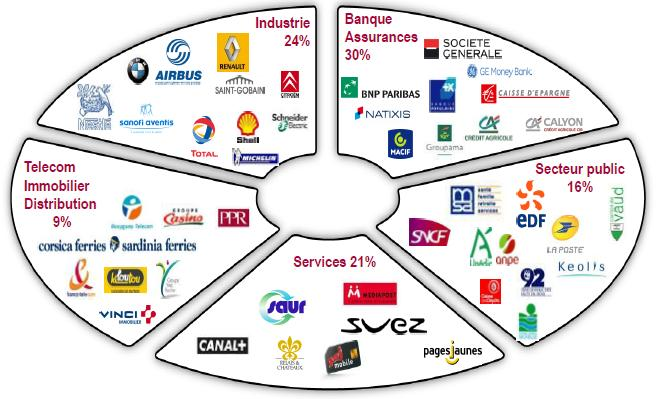
\includegraphics[width=0.7\textwidth]{assets/clients.jpg}
	\caption{Répartition des clients par secteur }
\end{figure}


\subsection{Evolution et positionnement}
Le groupe a affiché un chiffre d’affaires de 158.1M d'euros en 2012, pour un résultat net en progression à
4.5M d'euros. Ces résultats placent l’entreprise dans les 30 premières SSII en France en termes de chiffre
d’affaire. Si l’entreprise n’a pas le volume d’activité des très grandes SSII telles CapGemini, Atos ou
CGI (ex-logica), son positionnement technologique et sa volonté de fidélisation des clients lui ont permis au
cours des dernières années de remporter des marchés de la région bordelaise devant ces mêmes
entreprises. La diminution du chiffre d’affaires des deux années passées s’explique principalement
par un recentrage des activités du groupe et doit être relativisé par une progression du résultat net.




\begin{figure}[h!]
	\centering
	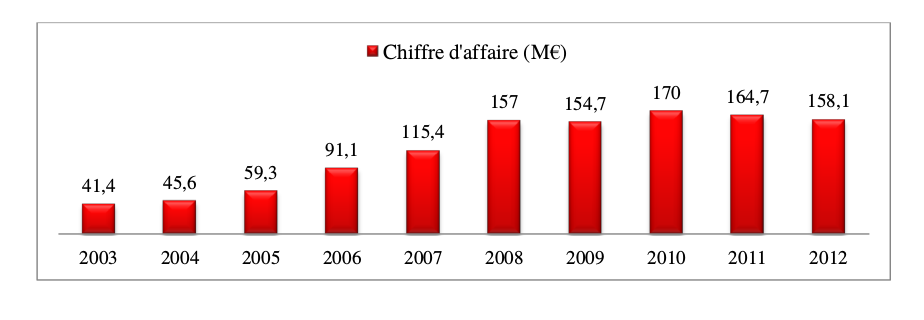
\includegraphics[width=0.7\textwidth]{assets/evol_ca.png}
	\caption{Evolution du chiffre d'affaire}
\end{figure}






\newpage






\section{Cellule d'expertise technique}

Dès le début de mon stage, j'ai été integré à la cellule d'expertise technique. Cette cellule unique dans chaque Agence, étant composé d'une poignée d'ingénieurs est utile à l'ensemble de l'agence pour : 

\begin{enumerate}
	\item La mise en place et maintien des environnements de développement, l'intégration continue
	\item La mise en place de référents techniques pour les développements
	\item Les revues de code 
	\item Les revues de conception et modélisation d’applications
	\item Dans le cadre d’intégration continue : audit de la performance du SI, analyse du temps de réponse et de la capacité de tenue de charge, identification des points de contention.
	\item Le transfert de compétences, par le biais de formations, workshops, entretiens de recrutements, etc.
	\item Assure la veille technologique. 
\end{enumerate}

C'est donc avec cette équipe que j'ai travaillé pendant les 3 mois de stage. 

\begin{figure}[h!]
	\centering
	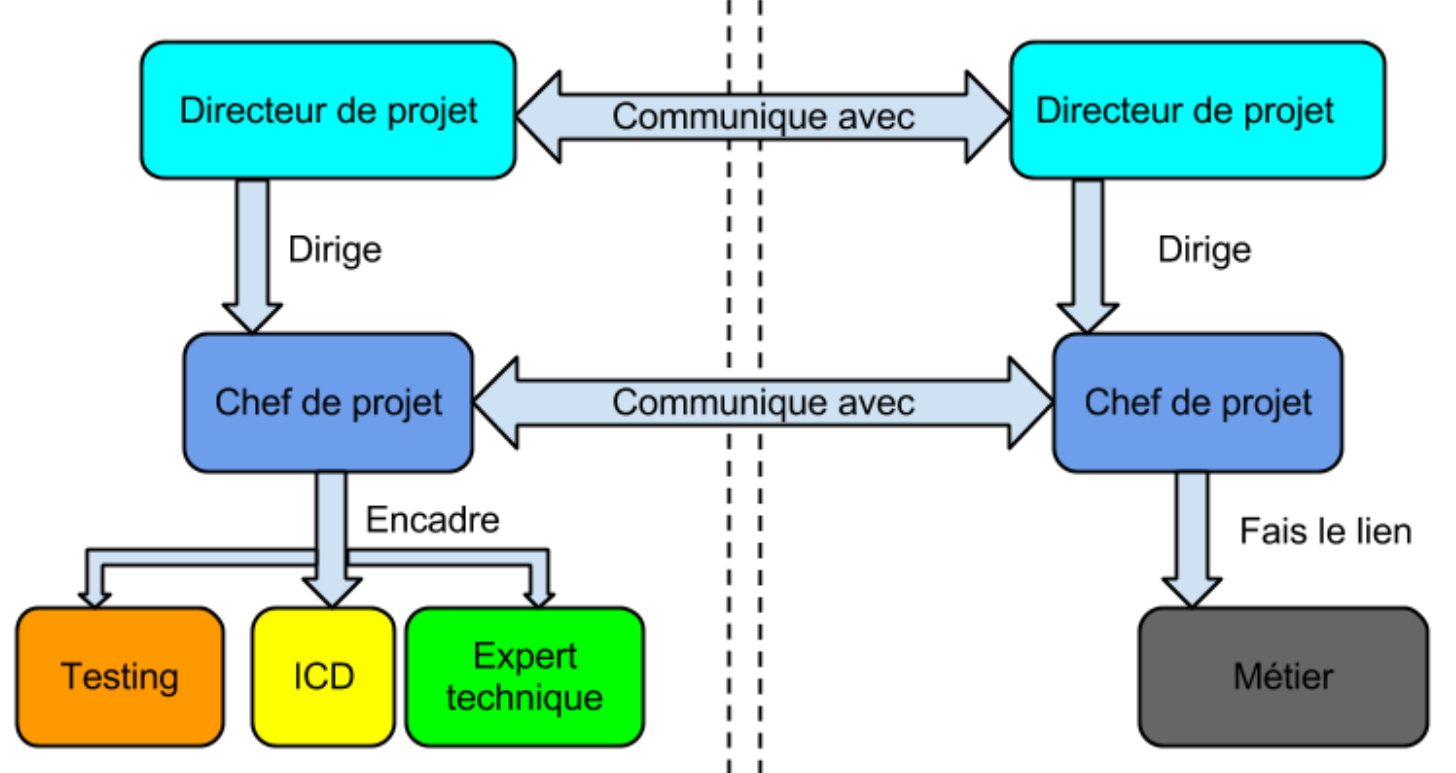
\includegraphics[width=0.7\textwidth]{assets/expert_orga.png}
	\caption{Rôle de l'expertise technique sur un projet. La partie droite représente le client.}
\end{figure}




\newpage



\chapter{Seating Plan}

L'application \gls{seating-plan} à traduire par plan officiel ou plan des bureaux, est un applicatif permettant d'avoir la répartition des bureaux, employés et téléphones sur les différents batiments de l'agence de Pessac. \\ 
Cet outil est utilisé par les directeurs de projets, directeur des ressources humaines pour leur permettre de gérer le capital humain. 


\section{Analyse des besoins}
Cette application déjà déployée en production, présente une ergonomie assez archaïque ainsi qu'une conception assez peu maintenable. \\


\begin{figure}[h!]
	\centering
	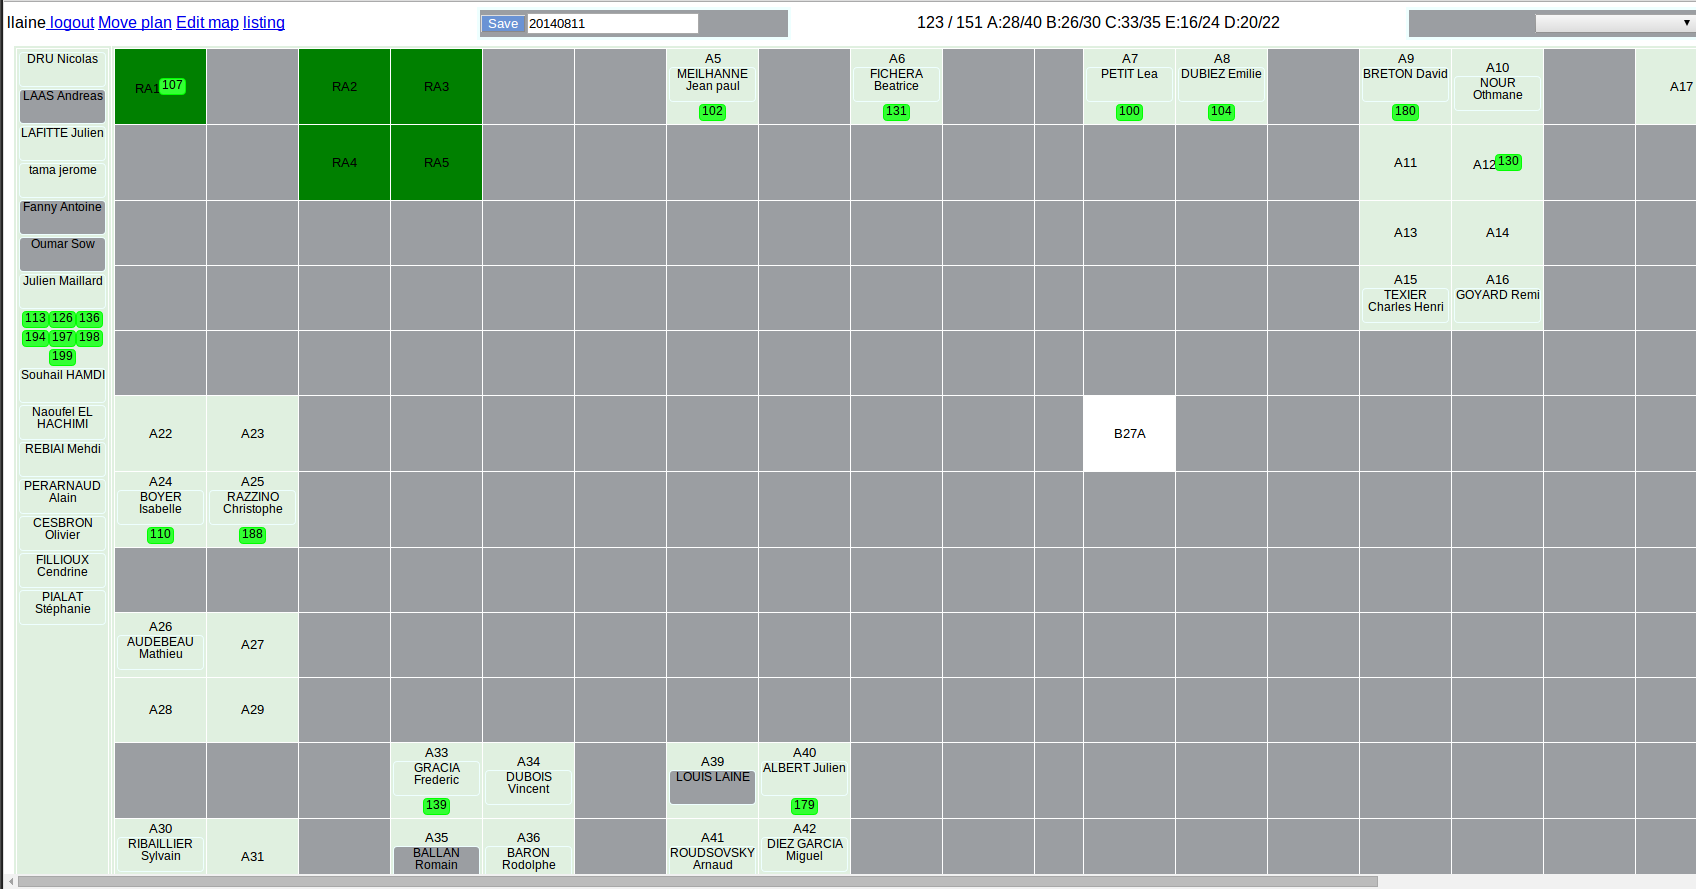
\includegraphics[width=1\textwidth]{assets/screenshot/old_seating.png}
	\caption{L'ancien seating}
\end{figure}

En réalisant l'état des lieux de l'application existante, j'ai pu déterminer qu'elle était écrite en \textbf{\gls{PHP}}, herbergée en local sur l'intranet de la société par le biais d'un server \textbf{\gls{Apache}} tournant sur une \gls{VM} \textbf{\gls{Debian}}. Aussi aucune base de données n'était présente pour effectuer la persistence. L'ensemble des données provenait de fichiers textes, aggrémentés à la main par le \gls{CTO}.  


\subsection{Problèmatiques}
Mon maitre de stage désireux d'améliorer cette application m'a demandé si j'avais dans un premier temps, la possibilité de corriger les quelques bugs présents et dans un second temps, de réaliser des améliorations sur l'existant. Etant donné l'état de l'applicatif déjà présent, j'ai décidé de repartir de zéro. 
\jumpOne
Il fallait déterminer quelles allaient être les contraintes pour ce projet. Toute la difficulté résidait dans la compréhension des attentes, pour réaliser un applicatif répondant au mieux aux besoins et ne pas livrer un outil en recul par rapport à la version précédente. 
\jumpOne
J'ai donc demandé à mon maitre de stage pour avoir quelques spécifications. 

\begin{itemize}
	\item L'application doit être écrite en PHP.
	\item Elle doit être accessible par tout le monde, mais en fonction de la personne se connectant octroyer un certain nombre de droits plus ou moins permissif sur les actions possible à réaliser.
	\item L'application doit être en mesure de gérer les différents plans par une interface de gestion avancée coté client. 
	\item Elle doit permettre de gérer le listing des employés, téléphones et bureaux.
	\item Elle doit permettre de gérer dynamiquement les différents bâtiments, pouvoir les activer/désactiver dynamiquement. 
	\item L'applicatif doit gérer un niveau de rôle spécifique à chaque utilisateur/groupe d'utilisateur. 
	\item En fonction du rôle octroyé par l'application, l'utilisateur doit avoir la possibilité de réaliser des sauvegardes des plans (pour tester par exemple une disposition particulière). En revanche, seule la dernière sauvegarde réalisée par un administrateur prévaudra sur l'ensemble des autres et c'est celle qui sera affiché par défaut. 
	\item L'applicatif, devra persister les données dans une base \gls{MySQL} et à partir de celle-ci fournir un ensemble de statistiques. 
	\item L'application devra embarquer une fonctionnalitée dite de \textbf{\gls{capacity-planning}} (gestion de la capacité), qui permettra à SQLI de garantir la qualité de service en alignement avec les besoins métiers. Cette activité de gestion de capacité sera ainsi composé d'une surveillance sur le long terme de l'ensemble du parc physique afin d'éviter le dépassement d'effectif d'une manière globale sur l'agence ou d'une manière détaillée sur un étage en particulier. 
\end{itemize}
 
\section{Conception et développement}
\subsection{Conception}
Etant donné le besoin de réactivité, j'ai donc choisi de réaliser une application se basant sur une \gls{client-serveur}. 

Le dialogue se fait donc de manière \gls{asynchrone} entre les deux couches et l'utilisateur n'est à aucun moment "bloqué" par le chargement d'une page. Une interface très réactive peut ainsi être mise en place par le biais de cette architecture. 

Pour uniformiser les transferts entre le client et le serveur le \gls{W3C} préconise l'utilisation d'une \gls{API} dite \gls{REST} qui est un style d'architecture. 

Cette \gls{API} \gls{REST}, me permet de faire l'interface entre la partie cliente et serveur. 

\begin{figure}[h!]
	\centering
	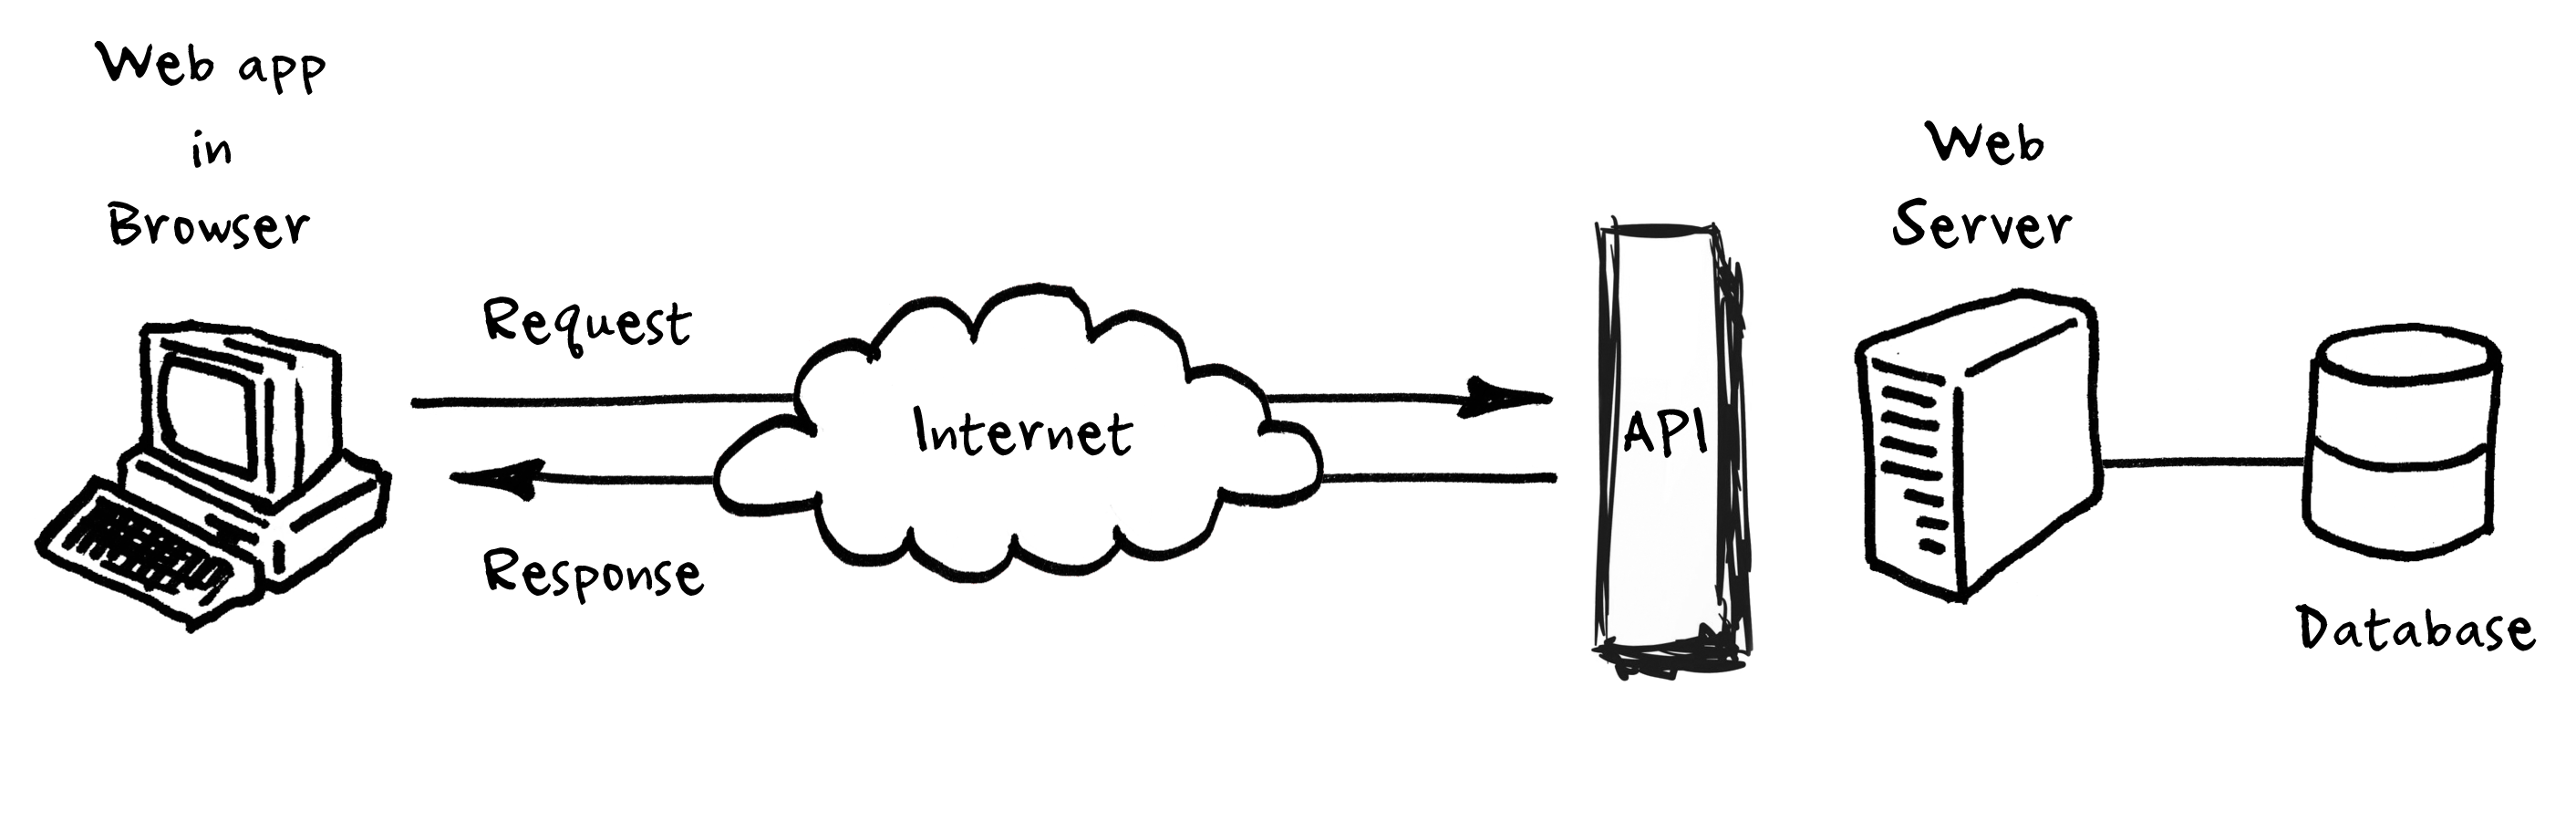
\includegraphics[width=1\textwidth]{assets/rest.png}
	\caption{Fonctionnement d'une API}
\end{figure}

\newpage
D'une manière générale ce type d'architecture permet de  
\begin{itemize}
	\item Découper les responsabilités entre le client et le serveur, pour permettre au deux d'évoluer indépendamment. 
	\item De libérer l'état de chaque requête. Celle-ci doit contenir toutes les informations nécessaires pour permettre au serveur de comprendre la requête, sans dépendre d'un contexte en particulier, ce qui permet d'économiser la puissance serveur nécessaire. 
	\item D'uniformiser l'interface avec des règles prédifinies simplifiant largement les échanges. 
\end{itemize}
Le \gls{framework} utilisé coté serveur utilise, une architecture spécifique, le \textbf{MVC}.
C'est un standard pour la création d'applicatif web, le \textbf{M}odèle \textbf{V}ue, \textbf{C}ontroller. 
\jumpOne
Ce modèle est destiné à répondre à des problèmatiques d'architecture d'application web. En effet, lors du développement d'une application web, ou d'une autre application, il est possible de ne pas suivre de pattern pour développer l'architecture. Seulement, l'application va très vite devenir instable car aucune séparation des responsabilités ce qui est assez compliqué à débuguer et à maintenir.
\jumpOne 
C'est ainsi que pour créer des applications web le \gls{MVC} s'est imposé comme standard de fait en une architecture permettant de séparer distinctement chaque logique d'une application en trois catégories.  
\begin{description}
   	\item[Le modèle] : Representant le coeur véritable de l'application, il va décrire les données manipulées par l'application. Il dialogue avec la base de données. Cette partie ne s'occupe pas de la présentation
   	\item[La vue] : Cette partie a comme tâche de présenter les résultats renvoyés par le modèle. Cette couche interagit également avec l'utilisateur et les différents évenements qu'il peut provoquer. 
   	\item[Le controller] :  Le controller prend en charge l'ensemble des traitements entre la vue et les modèles. Il va se charger de l'ensemble des évenements, déclenchés par la vue. 
   \end{description}   

\begin{figure}[h!]
	\centering
	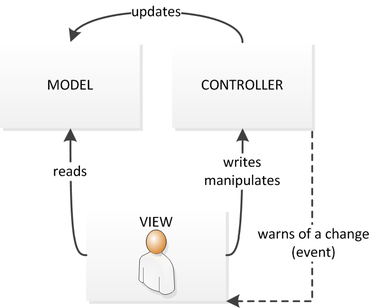
\includegraphics[width=0.6\textwidth]{assets/mvc.png}
	\caption{Fonctionnement du MVC}
\end{figure}

Cette architecture très claire permet également, aux autres développeurs qui vont reprendre mon application, de comprendre plus facilement son fonctionnement. 





\newpage





\subsection{Développement}
Pour mettre en oeuvre cette architecure, j'ai du choisir les outils à utiliser pour chaque partie. 

\begin{minipage}{0.5\textwidth}
	\begin{figure}[H]
		\centering
		
\includegraphics[width=0.4\textwidth]{assets/symfo.png}
		\caption{Logo de Symfony}
	\end{figure}
\end{minipage} 
\hfill
\begin{minipage}{0.45\textwidth}
	Coté serveur, mon dévolu se jeta sur \textbf{Symfony}, qui est un \gls{framework} \gls{MVC} écrit en PHP 5 ayant largement fait ses preuves, permettant de faciliter et d'accéler le processus de développement, se basant sur un ensemble de bonne pratique et de sucroit embarquant en natif le principe d'architecture \gls{REST}.
\end{minipage}

\begin{minipage}{0.5\textwidth}
	\begin{figure}[H]
		\centering
		
\includegraphics[width=0.5\textwidth]{assets/angular.png}
		\caption{Logo de AngularJS}
	\end{figure}
\end{minipage} 
\hfill
\begin{minipage}{0.45\textwidth}
	Coté client, je décidais de choisir le très à la mode \gls{framework} JavaScript \textbf{AngularJS} porté par Google, pour son architecture \gls{MVVM}, spécialement conçue pour des "web-app" ultra réactives, ce qui est en parfaite adéquation avec le futur seating-plan.  
\end{minipage}
\jumpTwo
La première difficulté rencontrée lors du développement, fut de faire communiquer les deux parties. En effet, Symfony en natif embarque un système de vue propre au \gls{framework}, qui au premier abord semble difficile de ne pas utiliser.  
\jumpOne
Après une recherche approfondie sur internet, je décide donc de chercher une solution pour faire dialoguer les deux couches d'une manière propre et évolutive. 
\jumpOne
Au bout de quelques heures, j'ai trouvé une solution et j'ai pu commencer à développer.

Ma découverte potentiellement qualifiée de "hacking" dans le sens ou l'on détourne le fonctionnement de quelque chose (et non pas l'autre définition parfois utilisé à tort comme synonyme de "piratage informatique"), j'ai également décidé en parallèle du stage, d'écrire un article sur un site spécialisé pour diffuser ma trouvaille, ce qui pourra potentiellement aider d'autre personnes qui comme moi ont recherché une solution sur internet, en vain. 

\href{https://medium.com/@llaine/operate-with-harmony-symfony2-angularjs-283b641d3b05}{Lien vers \textbf{l'article} (rédigé en Anglais)}





\newpage





\subsection{Gestion de projet}
\subsubsection{Agile}
SQLI étant certifié CMMI niveau 3, l'ensemble des pratiques utilisées pour gérer des projets suivent une \gls{guideline} bien définie. 
Concernant donc le développement de projet informatique, l'entreprise utilise une approche \emph{Agile}. 
Cette méthode s'oppose aux méthodes classiques qui spécifie et planifie avec le client dans les détails l'intégralité du produit avant de le développer. 
Le client va plutôt élaborer sa vision du produit à réaliser ainsi que la liste des fonctionnalités et des exigences à développer. L'équipe de développement va par la suite sélectionner une portion des exigences à réaliser dans une portion de temps courte appellée \textbf{itération}. 
Chaque itération inclut des travaux de conception, de spécification fonctionnelle et technique quand c’est nécessaire, de développement et de test. A la fin de chacune de ces itérations, le produit partiel mais utilisable est montré au client. Ce dernier peut alors se rendre compte par lui même très tôt du travail réalisé, de l’alignement sur le besoin. L’utilisateur final quant à lui peut se projeter dans l’usage du produit et émettre des feedbacks précieux pour les futures itérations. La visibilité ainsi offerte est clef. Cette transparence peut également apporter davantage de confiance et de collaboration dans la relation client/fournisseur. Les risques quant à eux sont levés très tôt.  \\

En opposition à la méthode Agile, on peut trouver par exemple le schéma de développement en V.
\subsubsection{Cycle en V}

\begin{figure}[H]
	\centering
	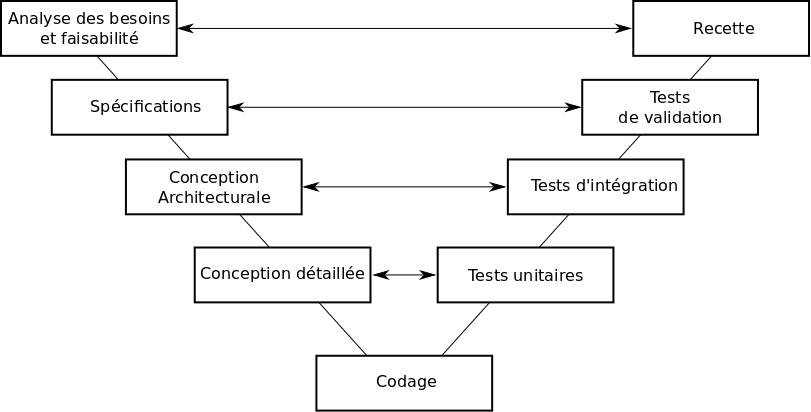
\includegraphics[width=1\textwidth]{assets/cycle_en_v.png}
\caption{Cycle en V}
\end{figure}
Ce modèle, est utilisé pour limiter au maximum la regression du projet en cas d'anomalie.  
On peut y distinguer trois grandes parties. 
\begin{itemize}
	\item Phase de conception
	\item Phase de codage 
	\item Phase de validation 
\end{itemize}
Chaque étape découle de la précédente ce qui diminue les risques sur le projet. 

C'est en suivant l'approche \emph{Agile} que j'ai réalisé le seating-plan.

\newpage






\subsubsection{Modèle de données}
Après avoir configuré et mis en place l'environnement, il fallu déterminer un modèle de données pour la persistence de celle-ci. 
\begin{figure}[h!]
	\centering
	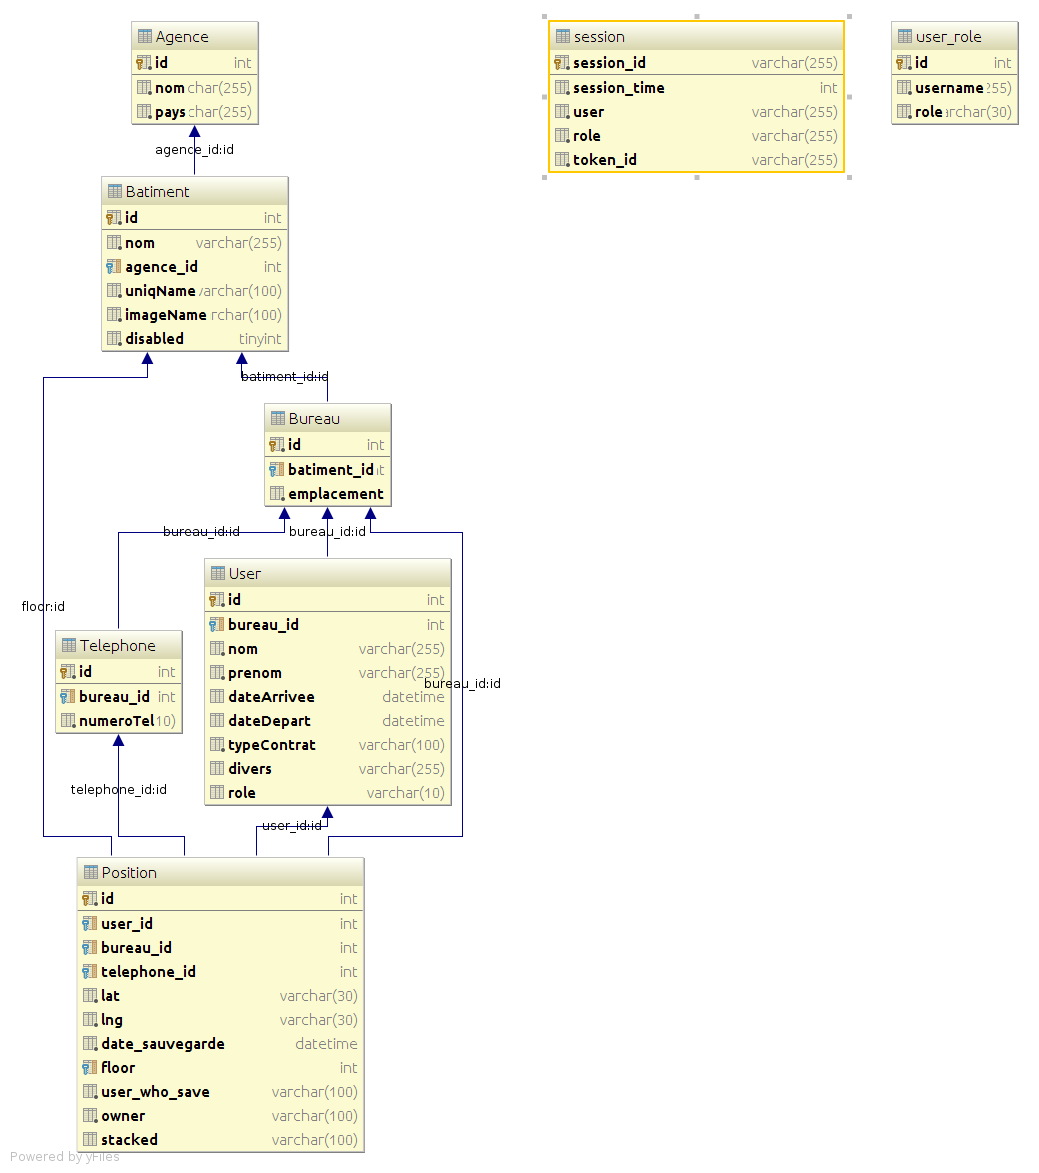
\includegraphics[width=1\textwidth]{assets/diagram.png}
	\caption{Modèle de base de données}
\end{figure}

Etant donné que Symfony se base sur un \gls{orm} pour faire le lien avec la base de données, le modèle objet sera exactement le même que celui de la base de données. 





\newpage





L'ORM qui signifie en anglais \textbf{object relational mapping} est une technique de programmation, qui permet d'avoir un modèle objet à partir d'une base de données relationnelle, en définissant des correspondances entre cette base de données et les objets du langage utilisé. Par exemple, les requêtes ne s'effectue plus en SQL mais en DQL (Doctrine Query Language) et non plus sur des tables contenant des champs, mais sur des objets contenant des propriétés.

Une fois le \gls{framework} configuré, j'ai pu commencer la phase de développement, utilisant GIT comme serveur de \gls{versionning} pour m'aider à sauvegarder mon code. 

\subsection{Capacity planning et interface gestion avancée}
\subsubsection{Capacity planning}
Une des fonctionnalités intéressantes à implémenter fût la mise en place du \gls{capacity-planning}. 
\jumpOne
En français gestion de la capacité, qui permet à SQLI de garantir la qualité de service en alignement avec les besoins métiers. Cette activité de gestion de capacité est ainsi consitutée d'une surveillance sur le long terme de l'ensemble du parc physique afin d'éviter le dépassement d'effectif d'une manière globale sur l'agence ou d'une manière détaillé sur un floor en particulier.
\begin{figure}[h!]
	\centering
	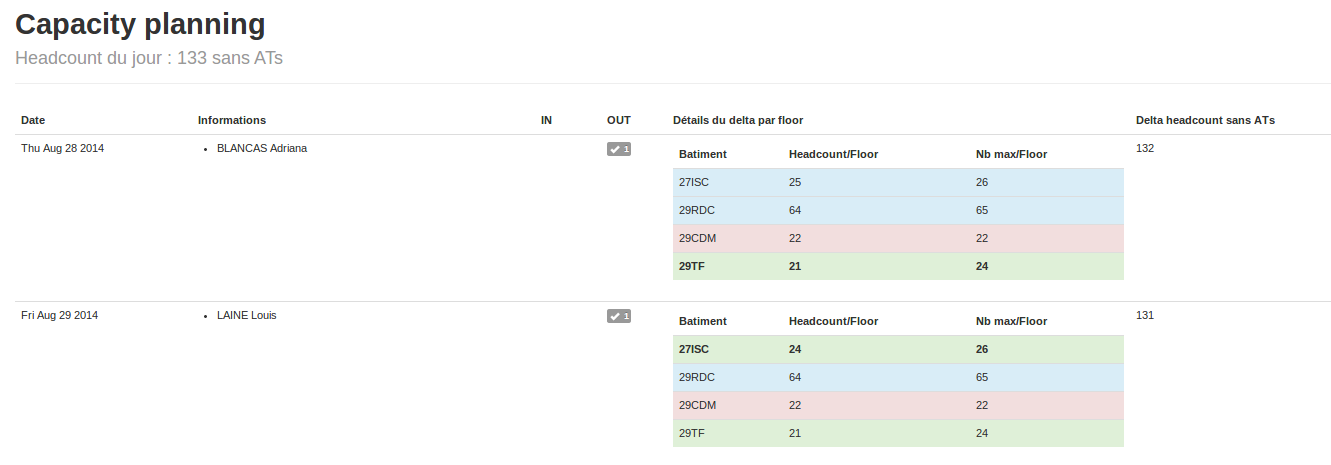
\includegraphics[width=1.1\textwidth]{assets/screenshot/capa_planning.png}
	\caption{Capacity planning actuellement en production}
\end{figure}

Ainsi, pour chaque date d'arrivée/départ d'une personne de l'entreprise le système est capable de donner la variation du nombre total de personnes présentes physiquement sur l'agence et de détailler ce chiffre sur l'ensemble des bâtiments activés dans l'application. \\
Sur l'exemple ci-dessus on peux constater, qu'au 28 août 2014, une personne s'en va du batiment \textbf{29TF}. De même pour le 29 ou une personne part du \textbf{27ISC}, libérant un bureau ramenant le nombre de places libre à un chiffre plus large. \\
L'utilisation d'un code couleur, permet de savoir rapidement si la marge restante est acceptable ou non.
\jumpTwo
Les managers vont pouvoir ainsi avoir une vision sur les mois à venir des différents bâtiments, qu'ils doivent gérer.

\subsubsection{Interface de gestion avancée}
La clé de voute de l'application, étant basée sur la réactivité, la gestion des différents plans ne pouvait se faire sans incorporer un système intuitif et agréable pour l'utilisateur. 

\begin{figure}[h!]
	\centering
	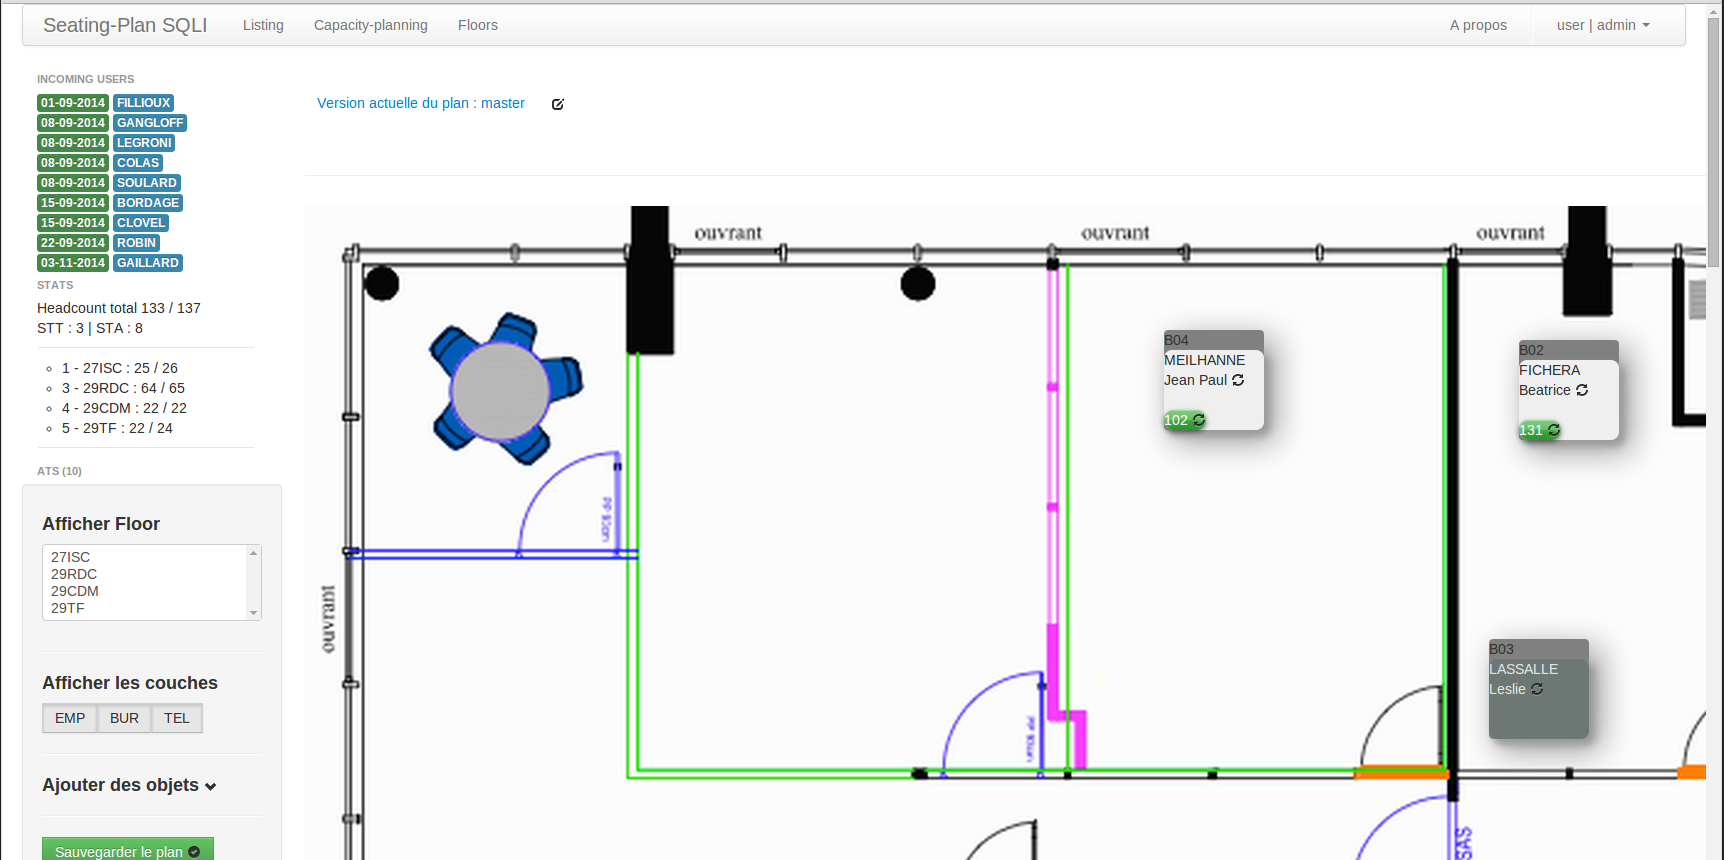
\includegraphics[width=1\textwidth]{assets/screenshot/design.png}
	\caption{Design du nouveau seating-plan}
\end{figure}
C'est ainsi que j'ai développé une sorte de mini \gls{framework}, basé sur \gls{jQuery UI} et le \gls{drag'n'drop} pour gérer toutes les interactions avec l'utilisateur. 
A l'aide d'une barre d'outils affichée sur le coté, l'utilisateur peux ajouter dynamiquement des objets sur les plans, qu'il va pouvoir faire glisser à un endroit spécifique. 
De même le système reconnaît les propriétés des différents objets qu'il est possible de manipuler. On pourra donc assigner un utilisateur à un bureau, avec des téléphones par exemple ce qui va afficher un plan complet  permettant d'avoir une idée du placement des employés et s'ils disposent de téléphones à proximité.  

Une fois le plan défini, l'utilisateur peut alors sauvegarder l'état actuel de ses modifications, figeant ainsi l'ensemble des objets. 
On peut ainsi arriver à gérer des étages, contenant beaucoup d'objets assez simplement 

\begin{figure}[h!]
	\centering
	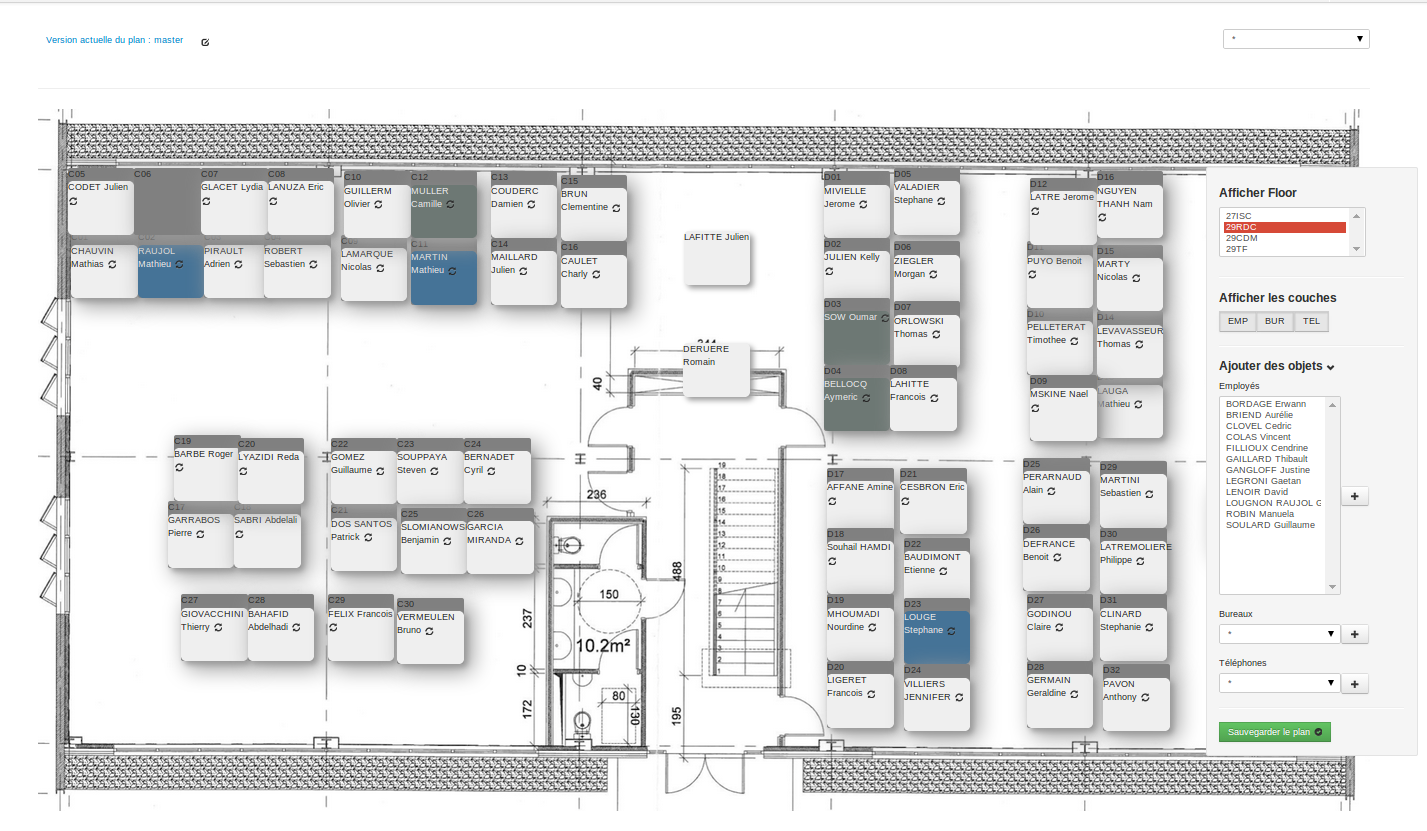
\includegraphics[width=0.9\textwidth]{assets/screenshot/plan_global.png}
	\caption{étage contenant beaucoup d'objets}
\end{figure}


\newpage





\section{Continuous integration}

Une fois l'application au stade d'une première version stable, j'ai procédé à la mise en production où mettre l'application en ligne. \\  
\jumpOne
Au début, j'ai tenté le déploiement à la main, par le biais d'un terminal, d'une session \gls{SSH} sur la machine serveur et de quelques script Shell. \\
Mais ce procédé n'étant pas en règle avec les bonnes pratiques de l'entreprise, j'ai vite changé pour utiliser une méthode différente, vivement recommandée par les experts techniques autours de moi. \textbf{L'intégration continue}.
\jumpOne
En effet dans le cadre d'une certification CMMI niveau 3 impliquant des méthodes d'extrême programming, SQLI utilise en interne une plateforme d'intégration continue, se basant sur \gls{Jenkins}. 
Cette plateforme va permettre aux développeurs de pouvoir déployer leurs applications, d'une manière automatisée et industrielle en incorporant un certains nombre de règles que le projet doit respecter pour être mis en production.

\begin{figure}[h!]
	\centering
	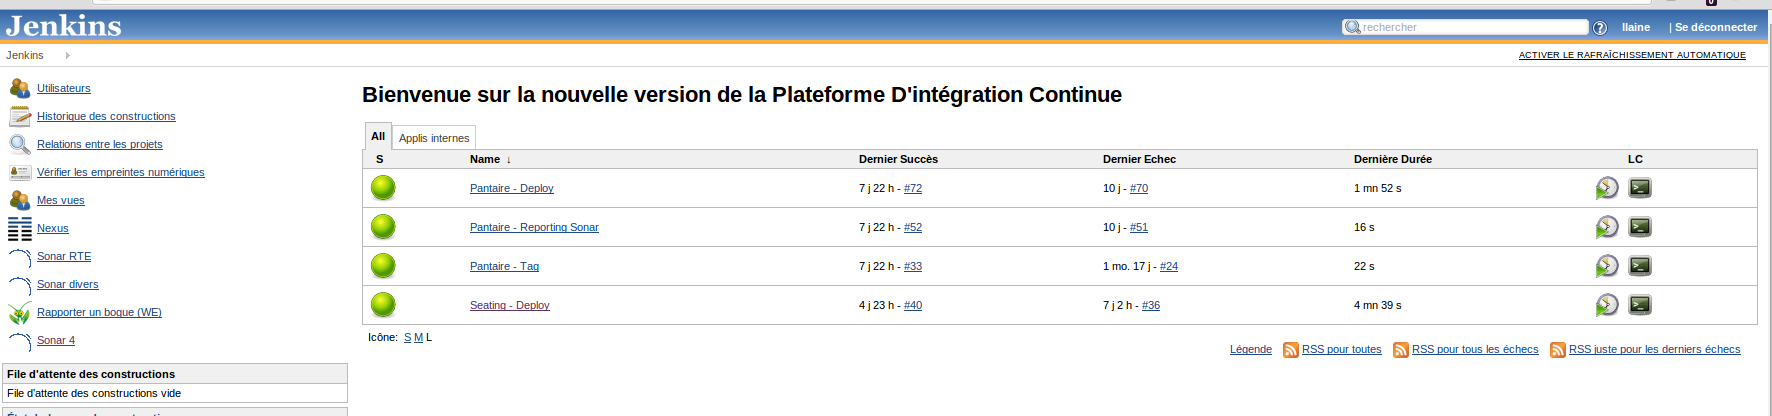
\includegraphics[width=1\textwidth]{assets/screenshot/jenkins.png}
	\caption{Capture d'écran du logiciel}
\end{figure}

A l'aide de \gls{Jenkins}, j'ai pu apprendre à déployer mon application de manière industrielle, par le biais d'un processus relativement simple et d'un script en Shell Unix faisant tout le travail à ma place me permettant d'avoir une solution automatique, reproductible et assez simple à éffectuer même pour une personne n'étant pas développeur. 
\jumpOne
Voici un exemple du script que j'ai utilisé pour effectuer la mise en production. 
\begin{lstlisting}[language=bash, caption=deploy.sh]
#!/bin/bash
...

setupRight(){
	cd ${APP_DIR}
   	#checkCache	
	rm -rf app/cache/*
	# Set right to cache/log folders
	chown mantis.www-data -R app/cache/
	chown mantis.www-data -R app/logs/
	chmod 775 -R app/cache/
	chmod 775 -R app/logs/
	echo "[i] Setup right ... "
}

# Clear the cache
clearCache(){
    cd ${APP_DIR}
    echo "Clearing cache for ${TARGET}  env"
    if  [[ ${TARGET} = "prod" ]]; then
        # Clear cache
        php app/console cache:clear --env=prod

        # Setting right
        setupRight
    else
        php app/console cache:clear
    fi
}

fetchLastVersion(){
    echo "[i] Fetching last version .."
    cd ${APP_DIR}
    git archive --format=tar --remote=git@10.33.33.15:llaine/seating.git ${VERSION} > archive.tar
    checkArchive
    tar -xf archive.tar
}

cleanUp(){
    echo "[i] Cleanning old repo ... "
    cd ${APACHE_DIR}
    sudo rm -rf ${APP_DIR}
    #echo "cd $APACHE_DIR && rm $APP_DIR"
    mkdir ${APP_DIR}
}


echo "[i] Deployement Seating.SQLI V ${VERSION}:${TARGET}"

usage # Checkin usage

checkEvt # Checking environnement

cleanUp # Cleaning folder in order to receive the new version

fetchLastVersion # Fetching last version

#setupRight # Setup good rights for the cache && logs folder

clearCache # Clear cache

echo "[i] Restarting server ... "

sudo service apache2 restart

...

\end{lstlisting}

Après lecture du code, on constate que le script éxecute toute les commandes qu'une personne fait de manière classique.
\jumpOne
En utilisant cette méthode, j'apprend d'une part de nouveaux outils qui me permettront d'être plus efficace sur le terrain dans le cadre de mon futur métier et d'autre part me permet de livrer un travail plus profesionnel, sur lequel il est très facile de faire des mise à jours, \gls{patch} et autres correctifs. Les autres experts techniques présent dans la cellule peuvent également reprendre mon code, dans le cadre d'évolution ou de correctifs et déployer de nouvelles versions facilement sans être bloqué par une quelconque manipulation dont moi seul aurait eu la connaissance.  





\newpage





\section{Valeur ajoutée du projet}
\subsection{Bilan}
Ce premier projet chez SQLI, m'a permis tout d'abord de prendre mes marques avec la société, l'environnement autour de moi. Ayant été seul à développer cette application, j'ai mis en place ma propre méthode de travail et développé les compétences de programmation apprises durant l'année.
La méthode utilisé s'articule en deux étapes.\\ 
Dans un premier temps, j'ai récolté des informations pouvant être utile à mon projet par le biais de petite réunion avec mon tuteur. Et dans un second temps une fois l'ensemble des spécifications en ma possession j'ai pu mettre en oeuvre ma méthode de travail, alternant des phases de développement intense, réalisant des objectifs fixés au jour le jour et des phases de revue de code ou des réunions. Celle-ci ajustée tous les jours pour arriver à une productivité optimale.


\subsection{Enseignements}
Réaliser ce projet m'a beaucoup appris, que ce soit dans la technique pure ou sur le côté fonctionnel. 
\jumpOne 
Du coté technique, j'ai pu apprendre sur la réalisation de projet en SS2I, j'ai pu me former sur des technologies nouvelles, très intéressantes et très utilisées sur le marché actuel. Etre plus au fait des standards, bonne pratiques et convention qu'il faut utiliser dans le monde du développement. \\ 
D'un point de vue fonctionnel, j'ai appris sur le fonctionnement de projet en SSII. En faisant partie de la cellule d'expert technique j'étais au coeur du fonctionnement de l'agence de Pessac. En assistant aux réunions hebdomadaires de suivi projets, j'ai pu mieux comprendre les notions étudiés durant l'année sur la gestion d'un projet puisque appliquées sur des situations réelles.   \\
D'un point de vue organisationnel, étant au contact au jour le jour avec les futurs utilisateurs de mon application, j'ai instauré un dialogue constant, me permettant de comprendre au mieux leurs attentes et de les traduire dans l'applicatif. \\
J'ai donc écouté d'une oreille attentive, leurs directives en assistant à des réunions diverses avec les différents protagonistes de l'agence Pessacaise. 
Avant de faire ce projet, je n'avais pas idée de l'importance qu'il pouvait y avoir à gérer constamment l'ensemble du parc physique dans une entreprise. Après avoir réalisé ce projet, je dirais que c'est indispensable, notamment étant donné la valeur très importante que représente le facteur humain dans une SSII.

\subsection{Recette}
Avant de déployer l'application, j'ai procédé avec mon maître de stage à une phase de recette. 
En amont du projet, une phase d'analyse des besoins et de faisabilité avait fourni des spécifications précises. Toute la difficulté fut de répondre par le biais de l'application au mieux à ces attentes.  
A la lumière des résultats obtenus ainsi que de l'appréciation de mon tuteur tout au long du projet, je pense que les objectifs ont été atteints pour l'entreprise. Il s'agissait en effet d'avoir un outil permettant de gérer consciemment les seating des différents bâtiments de l'agence de Pessac. 
\jumpTwo
Après avoir mis en production le seating-plan, mon tuteur de stage m'a orienté sur une autre mission, un projet en interne centré sur la performance des projets. 

 % Seconde partie.
 % Pantaire. 
 %
 %
 %%%%%%%%%%%%%%%%%%%%%%%%%%%%%%%%%%%%%%%%%%%%%%%%%%%%%%%%%%%%%%%%%%%%%%%%%%
 
 
\chapter{Pantaire}

\section{Analyse des besoins}
Pantaire est une application permettant de présenter sous une interface plus intuitive, l'ensemble des informations concernant les serveurs gérés par SQLI. 
Cette application, est déployée en interne ou chez les gros clients de la société. 
\jumpOne
En plus d'avoir accès aux informations serveurs, l'équipe d'expert désire pouvoir accéder aux indicateurs de performances des différents projets développés par l'entreprise. L'idée serait de présenter d'une manière condensée ces indicateurs, sur l'application Pantaire. 

\subsection{Problèmatiques}
Pour monitorer l'ensemble des projets qui sont développés, SQLI utilise un outil appelé \gls{SonarQube} qui permet de mesurer la qualité du code source en continu. 
Ce logiciel permet entre autres d'avoir un reporting précis sur différentes métriques comme :
\begin{itemize}
    \item Analyse statique de code
	\item Le taux de duplication de code dans un projet
	\item Le niveau de documentation
	\item Le respect de certaines règles de programmation 
	\item etc. 
\end{itemize}
L'agence de Pessac, peut ainsi garantir dans son développement et dans sa prise de décision, une certaine qualité de services directement chiffrable et tangible se basant sur des métriques (appelés \gls{KPI}) précises directement prises sur les différents projets. 
\jumpTwo
Cependant, certains indicateurs fourni par Sonar ne sont pas assez précis et pertinent et peuvent être faussés.
\jumpOne
Par exemple, lorsqu'on définit un certain niveau de contrainte à propos des règles de programmation à suivre durant un développement, il se peut que celle-ci soient sciement non-suivies pour des raisons propres à un projet. 
De plus concernant le code coverage (ou couverture de code, décrivant le taux de code source testé d'un programme permettant de mesurer la qualité des tests effectués), le taux peut atteindre une valeur illusoire, faussé par un nombre trop important de tests réalisés sur des getters et setters, n'ayant aucune valeur concernant la qualité du code.
\jumpTwo
Ma seconde mission pour ce stage, sera de créer un outil permettant de présenter d'une manière condensée et différente l'ensemble des métriques fournies par Sonar. 

\subsection{Specification}
Toute la difficulté réside dans la pertinence de la représentation de données. Les différents interlocuteurs clients auront accès à cet outil, et l'utiliseront pour avoir une idée de l'état des projets. L'applicatif doit être simple, intuitif et aller à l'essentiel. 
\jumpOne
Pantaire est une application, \gls{full stack} JavaScript. Elle utilise le même schéma d'architecture que le seating-plan, à savoir une \gls{client-serveur} ou les deux couches sont indépendantes et discutent entre elles. 
\jumpOne
Après quelques réunions avec les experts techniques m'indiquant leurs attentes j'ai pu réaliser une liste de spécification. 
\begin{itemize}
	\item L'outil doit être integré à un applicatif existant appelé \emph{Pantaire} et suivre le même modèle de développement que celui-ci. 
	\item L'outil doit permettre d'avoir l'ensemble des projets, pouvant être regroupés selon plusieurs propriétés. 
	\item Il doit permettre l'accès à l'historique de chaque métrique sur chaque projet.   
	\item Il doit intégrer une fonctionnalité de gestion de profil. Un profil correspond à un ensemble de métriques sélectionnées parmi lesquelles l'utilisateur va pouvoir appliquer une valeur plafond. Ainsi en sélectionnant un profil, l'utilisateur ne verra que les métriques qu'il a choisi sur les projets.
	\item L'outil doit intégrer une vision "de groupe", ainsi en fonction d'un profil et d'un groupe sélectionné avoir une vision globale de l'ensemble des projets et sur les métriques sélectionnées par le profil.    
	\item Il doit aller chercher de manière quotidienne les données dans \gls{SonarQube} et les persister dans une base de données, pour pouvoir les exploiter par la suite. 
\end{itemize}  
Concernant la partie front-end, comme dans le projet précédent j'ai utilisé \textbf{AngularJS}. Cependant concernant la partie back-end, j'ai utilisé \textbf{NodeJS} déjà présent sur l'application Pantaire.
\jumpOne
\begin{minipage}{0.5\textwidth}
	\begin{figure}[H]
		\centering
		
\includegraphics[width=1\textwidth]{assets/nodejs.png}
	\caption{Logo NodeJS}
\end{figure}
\end{minipage} 
\hfill
\begin{minipage}{0.45\textwidth}
	NodeJS est une plateforme basée sur le \gls{moteur V8} de Google, qui permet d'executer du Javascript coté serveur. Il a été créée pour répondre à des problématiques de montée en charge. Entièremment développé en C++, il commence à être beaucoup utilisé depuis quelques années.  
	\jumpOne
	Il embarque en natif une bibliothèque \gls{HTTP}, lui permettant de se comporter comme un serveur classique du type Apache, \gls{NGiNX}. Cependant, l'une des particularités de NodeJS est qu'il est un "langage" \gls{asynchrone}. 
\end{minipage}
\subsubsection{Asynchronous I/O}
D'une manière générale, nous sommes habitués à travailler de manière synchrone. Un programme, va appeler une instruction, qui va s'éxecuter et retourner une valeur. 
Une fois celle-ci terminée et une autre instruction s'effectuera et ainsi de suite. 
\jumpOne
Ce différent paradigme permet à la seconde instruction de s'éxecuter avant que la première soit terminée. Ainsi plusieurs instructions sont lancées sans se bloquer les unes aux autres. Le développement en suivant ce modèle est au début assez déroutant mais par la suite très intéressant, notamment grâce à sa rapidité d'éxecution.
\jumpOne

\begin{figure}[h!]
	\centering
	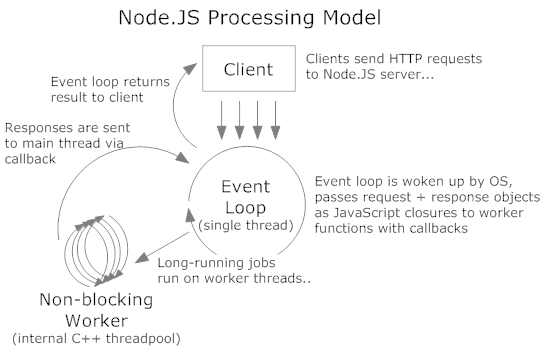
\includegraphics[width=0.7\textwidth]{assets/nonblockingio.png}
\end{figure}

Ce genre de modèle est très utilisé dans les système de gestion de base de données, comme Oracle ou SQL Server.





\newpage





\section{Réflexion sur le NoSQL (Not Only SQL)}
Concernant la persistence, vue la nature des données à aggréger et manipuler, une base de données \gls{MySQL} n'aurait pas été assez efficace en terme de performance, c'est donc que mon choix, dans le contexte de l'application Pantaire, c'est tout naturellement porté vers le \gls{NoSQL}. 
\jumpOne
\textbf{\gls{NoSQL}}, ce terme désigne l'ensemble des bases de données qui s'opposent à la notion relationnelle des \gls{SGBDR} classiques. Ces bases de données, proposent une alternative ou un complément aux fonctionnalités des bdd classiques. Les géants tels Google ou Facebook, ont mit au point ces solutions pour répondre à leurs besoins de scalabilité. 
\jumpOne
Le paradigme \gls{NoSQL}, très populaire ces dernières années, redéfinit totalement les bases de données. L'unité logique n'y est plus la table, les données ne sont pas manipulées avec SQL. Il rompt également avec les différents avantages propres au SGBD tels quel la cohérence des données de la base, les mécanismes de jointures, etc. 
En revanche là où le \gls{NoSQL} est intéressant c'est concernant la rapidité d'éxecution et le temps de réponse qui reste constant peu importe le nombre de données sauvegardées.
C'est également, concernant l'accès aux données qui s'effectue d'une manière assez simple, ce qui permet de manipuler assez facilement la masse de données persistée. 
\jumpOne
Il existe plusieurs types de base de données \gls{NoSQL}, nous allons nous intéresser ici uniquement à celle orientées documents. 
\jumpOne
L'ensemble des données, sont stockés sous forme de collections (l'équivalent des tables en SQL). Chaque collection, contient des documents (l'équivalent des enregistrement en SQL).


% Utilisation de JavaScript pour le lstlisting
\lstset{
   language=JavaScript,
   backgroundcolor=\color{lightgray},
   extendedchars=true,
   basicstyle=\footnotesize\ttfamily,
   showstringspaces=false,
   showspaces=false,
   numbers=left,
   numberstyle=\footnotesize,
   numbersep=9pt,
   tabsize=4,
   breaklines=true,
   showtabs=false,
   captionpos=b
}


\begin{lstlisting}[language=javascript, caption=Exemple d'un document JSON]
	
	{
	  "Subject": "Why NoSQL"  
	  "Author": "Lainé"  
	  "PostedDate": "19/01/2014"  
	  "Tags": ["NoSQL", "database", "scalability"]
	  "Body": "Today i'm going to talk about NoSQL ..."
	  "Comments": [
	  		{
	  			'date': '20/01/2014'
	  			'text' : 'Great post ! '
	  			'authorId': '02356'
	  		}

	  ]
	}
\end{lstlisting}  
La base de données utilisée dans ce programme s'appelle \textbf{\gls{MongoDB}}, l'une des plus populaire base de données \gls{NoSQL}, sous licence open source actuellement en version 2.6.

\subsection{Pourquoi les bases NoSQL sont elles intéressantes ? }

\begin{itemize}
	\item La \textbf{productivité}. Le temps passé à concevoir et à maintenir les bases de données relationnelles, avec le mapping objet correspondant, peut-être assez long en fonction du projet. Le \gls{NoSQL} peut proposer un modèle de données qui correspondra peut être mieux aux contraintes de l'application, impliquant moins de code à écrire et à débuguer simplifiant grandement les interactions avec la base de données.
	\item La \textbf{scalabilité}. Les bases de données relationnelles sont à la base conçues pour tourner sur une machine unique, cependant il est plus économique d'utiliser des clusters de petites machines, plus économiques, pour gérer beaucoup de données. La plupart des bases de données \gls{NoSQL} sont conçues pour être déployées sur des \gls{cluster} exploitant au mieux le \gls{big data}.   
\end{itemize}


\section{Développement}
Une fois l'ensemble des outils mis en place, j'ai pu commencer à développer le projet.

Sous la tutelle de Christophe Frézier, j'ai au fil des semaines implémenté des fonctionnalités, suivant l'architecture \gls{REST} et les bonnes pratiques mise en place pour ce projet. 
\jumpOne
En plus d'utiliser \textbf{NodeJS} coté serveur, j'ai utilisé un module appelé \textbf{Restify}, qui m'a permis de construire très facilement une \gls{API} \gls{REST}.   
\begin{lstlisting}[language=javascript, caption=Exemple d'utilisation avec restify]
(function(){
	var restify = require('restify');

	// Création d'un instance serveur
	var server = restify.createServer();

	// Pour une resource
	server.get('/resource', function);
	server.post('/resource', function);
	server.put('/resource', function);
	server.delete('/resource', function);

	server.listen(8081, function(){
		console.log('Server listening at %s', server.url);
	});
})();
\end{lstlisting}

Le Javascript n'étant pas un language très contraignant concernant l'architecture à mettre en place, j'ai pu donc facilement créer ma propre architecture, déplacant d'un côté les modèles et de l'autre les logiques métiers dans un module à part. 


\newpage



Pour assurer les transactions avec la base de données noSQL, j'ai utilisé un librairie appelé \textbf{Mongoose} qui facilite largement l'utilisation avec \textbf{NodeJS}.

\begin{lstlisting}[language=javascript, caption=Exemple de définition d'un schema NoSQL]
var mongoose = require('mongoose'),
    Schema = mongoose.Schema;

module.exports = (function(){

    /**
     * @type {Schema}
     */
    exports.schema = new Schema({
        nom: String,
        metriques: [{
            key: String,
            value: String
        }]
    });


    return mongoose.model('Profile', exports.schema);

})();
\end{lstlisting}
\begin{lstlisting}[language=javascript, caption=Exemple d'accès aux données]
/**
 * GET all the profile from the DB
 * @param req
 * @param res
 */
 exports.getAllProfile = function(req, res){

    res.setHeader('Access-Control-Allow-Origin', '*');

    modelDispatcher.Profile.find().exec(function(err, lesProfiles){

        handleErrors(err);

        displayDebug("Getting all the profiles");

        res.send(lesProfiles);

    });

};
\end{lstlisting}
On constate ici, qu'aucune requête de type SQL n'est utilisé, en effet \gls{MongoDB} pour accéder à ses données va utiliser des fonctions du type \textbf{find} ou \textbf{findOne}.
Ce type de requêtage est très semblable à celui d'une liste ou d'une collection ce qui permet de très facilement accéder aux données.
\jumpTwo
Tout au long de cette seconde mission, j'ai utilisé plusieurs outils plus ou moins nouveaux à ma connaissance me permettant d'enrichir ma méthode de travail.


\newpage



\subsection{Build pattern}   
Dans un soucis de gestion d'automatisation de production, le projet existant utilise des outils sur lesquels j'ai du me former pour être en conformité avec les conventions de développement.
\subsubsection{Grunt}
Pour automatiser les tâches j'ai utilisé \textbf{Grunt}, qui m'a beaucoup aidé à améliorer ma rapidité de travail. Nombre de tâches sont très répétitives dans le monde du développement logiciel, par exemple sur Pantaire, en fonction de l'environnement de déployement on désire pouvoir accéder à plus ou moins de contenu. Par le biais d'un fichier de configuration, on va assigner des variables qui seront en fonction de l'environnement de destination valorisées différement. 

\begin{lstlisting}[language=javascript, caption=Ex de configuration en fonction d'evt]
// Environnement de développelement 
"dev" : {
    "serverPort"        : "8081",
    "serverHost"        : "127.0.0.1",
    "zabbixUrl"         : "http://10.33.33.9/zabbix/api_jsonrpc.php",
    "zabbixUser"        : "zefi436nfez",
    // ...
}
"prod : {
    "serverPort"        : "8085",
    "serverHost"        : "127.0.0.1",
    "zabbixUrl"         : "http://10.33.33.9/zabbix/api_jsonrpc.php",
    "zabbixUser"        : "aa234grehix",
    // ...
}
\end{lstlisting}

Ces variables de configuration, sont utilisées dans l'ensemble de l'application. 
Changer l'ensemble de celles-ci dans tous les fichiers à chaque fois qu'on désire changer d'environnement serait une perte de temps énorme et les risques d'erreur seraient beaucoup plus grands.
\jumpOne
C'est là, ou Grunt va nous aider
En définissant une tâche particulière, l'outil va faire le travail à notre place et générer nos fichiers de configuration. 
Voici un exemple de définition de tâche.
\begin{lstlisting}[language=javascript, caption=Tâche de concaténation des fichiers]
// Exemple de définition
module.exports = function(grunt) {

  grunt.initConfig({
    replace: { // Nom de la tache
        dist: {
            options: { // Options
                patterns: [
                    { match: 'version', replacement: '<%= pkg.version %>' },
                    { match: 'title', replacement: '<%= pkg.name %>' },
                    { match: 'timestamp', replacement: '<%= grunt.template.today() %>' },
                    { match: 'serverPort', replacement: environment.serverPort  },
                    { match: 'serverHost', replacement: environment.serverHost },
                    { match: 'zabbixUrl', replacement: environment.zabbixUrl },
                    { match: 'zabbixUser', replacement: environment.zabbixUser },
                    // ...
                ],
                force: true
            }, // Fichier cibles 
            files: [
                {
                    src: [ './frontend/conf/confSkeletonFO.js' ], 
                    dest: './frontend/conf/generated_conf.js'
                },
                {
                    src: [ './backend/modules/conf/confSkeletonBO.js' ], 
                    dest: './backend/modules/conf/generated_conf.js'
                }
                ]
            }
        }
  })

  // Redéfinition de la tache défaut, pour qu'elle prenne en compte notre replacement.
  grunt.registerTask('default', ['replace'])
}
\end{lstlisting}
Désormais en lancant la commande \emph{grunt replace}, et en indiquant l'environnement cible mes fichiers vont tout simplement se modifier. 
\jumpOne
Il est possible de créer des tâches très différentes, comme par exemple celle de lancer des tests unitaires, créer une nouvelle version, etc. 



\subsubsection{Bower}
Dans la panoplie de l'automatisation de production Javascript, Bower est un autre module très intéressant. 
\jumpOne
Là où \textbf{Grunt}, nous permet d'automatiser, \textbf{Bower}, nous permet de gérer l'ensemble dépendances d'un projet.
Dans un souci de gain de temps et de factorisation, on évite de recoder à chaque fois tout ce dont on a besoin et on utilise des librairies tierce. 
Ainsi, lorsqu'on commence un nouveau projet on a tendance à copier-coller toutes les librairies qu'on désire utiliser à la main. 
On perd donc du temps et on risque de se retrouver face à des dépendances dépréciées ou manquantes. 
\jumpOne
C'est la ou Bower entre en jeu. 
En créant un fichier appelé \textbf{bower.json}, contenant l'ensemble des dépendances et en lancant une commande d'installation, le petit script va télécharger automatiquement celles-ci dans la version désirée. 
\begin{lstlisting}[language=javascript, caption=Exempe-type de fichier JSON]
{
    "name": "projet", // Nom du projet
    "dependencies": { // Les dépendances utilisées.
        "knacss": "latest",
        "html5shiv": "latest",
        "box-sizing-polyfill": "latest",
        "modernizr": "latest",
        "jquery": "1.10.2"
    }
}	
\end{lstlisting}
Ces outils, sont semblable à \textbf{Apache Maven} ou \textbf{Gradle} dans le monde Java. 
\jumpOne
Couplé à l'utilisation d'une plateforme d'intégration continue (utilisée également dans ce projet), on peux ainsi arriver beaucoup plus facilement à gagner en productivité, automatiser l'ensemble des tâches ingrâtes que peut apporter le développement et se concentrer uniquement sur la programmation. 
\subsection{GIT}
Dans le monde du développement informatique, lorsqu'on travaille à plusieurs sur le même projet et sur le même code source, on fait face à de nombreux problèmes.
Les modifications provoquant des bugs, une version sur une machine qui ne fonctionne plus sur une autre, l'historisation des versions et le code correspondant à chaque \gls{patch}, etc. En somme, beaucoup de problèmes, qu'il est possible de contourner à l'aide d'un logiciel de gestion de versions. 
Il va permettre de suivre l'évolution d'un fichier texte ligne par ligne. Il permet par exemple de sauvegarder en plus des modifications, la personne ayant modifié chaque fichier ainsi que la raison de cette modification. Il peut également fusionner deux versions d'un même fichier en évitant que l'une des deux versions soit écrasée. 
\jumpOne
Aussi bien dans le projet précédent que dans celui-ci, j'ai utilisé Git qui est un logiciel très puissant pour permettre le travail colaboratif. 
Chaque nouvelle fonctionnalité était enregistrée puis assignée à un commit ou une branche spécifique. De même lorsque je désirais pousser en production mon code, mergeant mon travail sur la branche master le travail était largement simplifié pour l'administrateur du code source qui pouvait très simplement voir chaque ligne de code que j'avais écrite y apposer un commentaire, qui pouvait être discuté par la suite.  


\section{Valeur ajoutée du projet}

\subsection{Bilan}
Le bénéfice d'avoir pu effectuer deux missions distinctes lors d'un même stage, m'a permis de développer compétences apprise durant l'année, devenant plus polyvalent dans ma démarche professionnelle et renforcer la compréhension du développement en SSII. 
\jumpOne
Ce second projet m'a également permis de prendre du recul avec le travail précédemment éffectué. Ayant progréssé dans la mise en oeuvre des outils, je comprend après coup les méthodes que j'aurai pu mettre en place dans la réalisation de ma première mission et le temps que j'aurai gagné en utilisant celles-ci. 

\subsection{Enseignements}
Sur le plan technique, en me formant à de nouvelles technologies, j'ai pu accroitre mes connaissances que ce soit en matière de base de données en utilisant le NoSQL ou encore sur la programmation serveur avec NodeJS.

Concernant la méthodologie de travail, j'ai beaucoup apprécié m'exercer à l'ensemble des opérations annexes à la programmation. Avant ce stage, je n'avais pas idée des avantages à utiliser les outils d'automatisation, d'intégration continue. C'est maintenant quelque chose d'incontournable que je vais m'efforcer d'utiliser dès que j'en aurais l'occasion.
\jumpOne 
De plus dans la manière de développer, ayant été sous la tutelle d'experts techniques durant toute la durée de ce second projet, ils m'ont transmit les bonnes manières, les conventions à respecter dans le développement me permettant de beaucoup progresser sur ce point.
\jumpOne
Et bien sûr d'un point de vue fonctionnel, j'ai pu m'instruire encore plus sur le fonctionnement d'une société et la gestion de projet. En participant à des réunions différentes du premier projet, avec des personnages différentes, j'ai agrandi mes découvertes sur les différentes synérgies qu'il peut y avoir entre les différentes entités constituantes de l'agence. Sur la manière dont SQLI utilise la méthode Agile ou le cycle de développement en V pour gérer ses projets, chaque étape me semble désormais plus simple, claire et précise.


% Conclusion
\chapter{Une expérience réussie} 
Ce stage de fin de licence très orienté technique, me permit d'aborder un certain nombre de technologies. La liberté que j'ai eu pour remplir mes fonctions que ça soit dans le projet seating-plan ou bien Pantaire est appréciable dans la mesure ou j'ai travaillé en interne et pas directement intégré à une équipe sur une ligne de production. Les délais à respecter y sont souvent courts et des résultats plus précis y sont attendus. A contrario, le manque de structure peut s'avérer être un obstacle. Il faut une bonne autonomie, de la rigueur de la régularité pour parvenir à mener de tels projets à bien. 
Le plus difficile fut le premier projet, ou il a fallu tout en s'adaptant au tout nouvel environnement, répondre au mieux aux attentes de mon maître de stage pour lui donner une application qui soit au plus proche de ses attentes. A la lumière des résultats obtenus ainsi que de l'appréciation de mon tuteur entreprise tout au long du projet, je pense que les objectifs ont été atteints pour l'entreprise. Il s'agissait en effet d'avoir un outil permettant de gérer consciemment le seating des différents bâtiments. 
Pantaire fût tout aussi intéressant, apportant son lot de surprise, de joie et de frustration. La mission était beaucoup plus précise que sur le seating plan et nécessitait une compréhension plus appropriée du problème. Ce second projet me permit d'élargir mon champ de compétence techniques, fonctionnelles et méthodologiques. 
\jumpOne
D'un point de vue plus personnel, j'ai tout particulièrement apprécié le cadre du stage. SQLI Bordeaux est un site dynamique où la communication est aisée et l'ambiance détendue.
Les différentes missions ont été intéressantes, exposant au maximum les compétences techniques tout en s'appuyant sur des besoins fonctionnels.
Les outils sur lesquels j'ai pu me former, AngularJS, NodeJS et le NoSQL, diversifiant mon panel d'outil à disposition.
Les notions plus gestion de projets mettant en oeuvre la méthode Agile ou le schéma développement en V, ou l'extrême programming, s'intéressant aux notions d'intégration continue. 
Enfin la proximité des experts techniques, présents pour m'aider lorsque j'en avais le besoin et présent pour m'apprendre de nouvelles notions, partageant leurs savoir. \\
Une expérience enrichissante tant sur le plan personnel que professionnel qui m'a permis de gagner en maturité dans mes méthodes de développement, d'avoir une approche différente sur les notions de gestion de projet ou de développement apprisent à l'université.


\chapter{Annexes}

\section{Sources}

\begin{itemize}
	\item \href{http://fr.wikipedia.org/}{Wikipedia d'une manière générale}
	\item \href{http://tex.stackexchange.com/}{Site d'entraide pour le langage LaTeX}
	\item \href{http://www.mongodb.org/}{Documentation MongoDB}
	\item \href{http://nodejs.org/}{Documentation NodeJS}
	\item \href{http://mongoosejs.com/}{Documentation Mongoose}
	\item \href{http://gruntjs.com/}{Documentation Grunt}
	\item \href{http://jenkins-ci.org/}{Documentation Jenkins}
	\item \href{http://bower.io/}{Documentation Bower}
	\item \href{https://angularjs.org/}{Documentation AngularJS}
	\item \href{http://fr.wikipedia.org/wiki/NoSQL}{Page wikipedia sur le NoSQL}
\end{itemize}



\section{A propos}
\begin{description}
	\item Rapport écrit sur un système libre GNU/Linux à l'aide de \LaTeX. 
	\item \href{https://github.com/llaine/internship-L3}{Code source du rapport}.
\end{description}



\printglossaries





\end{document}